\documentclass{article}

\newif\iflotteryneurips
\ifdefined\LOTTERYNEURIPS
  \lotteryneuripstrue
\else
  \lotteryneuripsfalse
\fi

\newif\iflotteryiclr
\ifdefined\LOTTERYICLR
  \lotteryiclrtrue
\else
  \lotteryiclrfalse
\fi

\iflotteryneurips
  \PassOptionsToPackage{numbers,compress}{natbib}
  \usepackage[main]{neurips_2026}
\else
  \iflotteryiclr
    \usepackage{times}
    \usepackage{iclr2026_conference}
  \else
    \usepackage[margin=1in]{geometry}
    \usepackage[numbers]{natbib}
  \fi
\fi

\usepackage{booktabs}
\usepackage{graphicx}
\usepackage{amsmath}
\usepackage{amssymb}
\usepackage{amsthm}
\usepackage{xcolor}
\usepackage{hyperref}

\newtheorem{proposition}{Proposition}

\newif\iflotteryincludeappendix
\ifdefined\LOTTERYMAINONLY
  \lotteryincludeappendixfalse
\else
  \lotteryincludeappendixtrue
\fi

\iflotteryincludeappendix
  \newcommand{\cifarmovementappendixref}{Appendix Table~\ref{tab:cifar-movement-stats}}
\else
  \newcommand{\cifarmovementappendixref}{the supplemental generated movement table}
\fi

\title{Winning Tickets Are Not Posterior Modes:\\
Evidence from Posterior Support and Magnitude Controls}

\author{Anonymous}
\date{\today}

\begin{document}
\maketitle

\begin{abstract}
The lottery ticket hypothesis suggests that dense neural networks contain sparse
subnetworks that can be trained in isolation when rewound to their original
initialization. A tempting Bayesian interpretation is that these tickets
correspond to posterior modes, or to posterior-basin supports. We turn this
interpretation into a pre-specified, falsifiable test: posterior-induced masks
must match IMP tickets better than local magnitude, dense-trajectory, and
pruning-process controls, not merely better than uniform random masks. Across
five-seed MNIST and Fashion-MNIST sparsity sweeps and a CIFAR-10 ResNet-20
epoch-1 rewind setting, fourteen posterior approximations---SGLD, SGHMC,
cyclical and parallel-tempered SGLD, SWAG, the Laplace family up to
joint-group full covariance, subspace HMC, and deep ensembles---fail this
stronger criterion. Posterior supports often beat random masks,
but they remain tied to chain-start magnitude, dominated by dense magnitude, or
closer to rewind controls than to IMP. Support-equivalence is graded rather than
binary: only a rank-128 Hessian-plus-diagonal Laplace crosses the mask-overlap
threshold, and even it fails the layer-sparsity and basin-count gates, so a
posterior account survives on one axis at one fidelity. We then give a positive
account of what winning tickets are: trajectory and pruning-process objects.
Dense-trajectory magnitude explains most of the fixed-mask training gap and a
process-selected IMP-only residual explains the rest, with an extensive battery
of process controls failing to substitute for it. This account is consistent
with axial-subspace views of IMP and inconsistent with a posterior-mode view.
Exact dense full-network full-covariance CIFAR posterior baselines remain an
open limitation.
\end{abstract}

\section{Introduction}

The lottery ticket hypothesis (LTH) states that a dense randomly initialized
network contains sparse subnetworks that can be trained to match the dense
network when reset to their original initialization \citep{frankle2019lottery}.
This result raises a basic question about the object discovered by iterative
magnitude pruning (IMP): is a winning ticket a combinatorial artifact of the
optimization trajectory, or does it reflect a deeper probabilistic structure of
the posterior over weights?

A Bayesian reading is attractive: SGD and its noisy variants connect to
approximate Bayesian inference \citep{welling2011sgld, mandt2017sgd}, and
Bayesian deep learning emphasizes that useful solutions are distributed
across broad posterior regions \citep{wilson2020bayesian,
izmailov2021posteriors}. If winning tickets correspond to posterior modes or
posterior-basin supports, LTH would be evidence for a selection view of
learning: pruning would reveal posterior structure already present in the
trained model.

This paper tests that interpretation directly. We ask:

\begin{quote}
Do posterior samples or posterior basins induce sparse supports that explain IMP
winning-ticket masks beyond dense magnitude, initialization magnitude, rewind
magnitude, chain-start magnitude, and pruning-process controls?
\end{quote}

The paper makes three first-class contributions.
\textbf{(i) A controlled negative empirical result.} We state the
posterior-mode explanation as a \emph{pre-specified}, falsifiable
support-equivalence claim---posterior-induced supports must beat local
magnitude controls, not just random masks, and mode/ticket distributions must
match in mask and function space---with the operational gates fixed before
the posterior runs. The gates are then evaluated across repeated
MNIST/Fashion-MNIST sweeps and fourteen CIFAR-10 ResNet-20 posterior
approximations (stochastic samplers, Laplace variants, SWAG, subspace HMC,
and direct mode/ticket probes), with a locked final-test confirmation that
matches three pre-registered numerical predictions. Support-equivalence is
\emph{graded} rather than binary: a single rank-128 Hessian-plus-diagonal
Laplace passes the mask-overlap axis while still failing the layer-sparsity
and basin-count axes.
\textbf{(ii) A positive trajectory and pruning-process account.} IMP
tickets are explained by dense-trajectory magnitude plus a process-selected
IMP-only residual rather than posterior-mode supports.
Proposition~\ref{prop:topk} formalizes why high-SNR posterior TopK masks must
track the chain-start magnitude support.
\textbf{(iii) A reusable posterior-vs-IMP audit framework.} The operational
support-equivalence gate, the fourteen-approximation harness, the
pre-registered locked-test protocol, and the surrounding audit suite are
released as a reusable testbed so other posterior families can be tested
against IMP tickets under the same operational contract. The release adds
a standing open-challenge protocol: third parties may submit any posterior
construction---including multimodal families we could not exhaust---and we
commit to re-running the unmodified gate and registering the outcome.

The conclusion is negative but scoped. Posterior masks beat random masks but
track the dense-checkpoint or chain-start magnitude support; chains that move
do so without moving toward the IMP ticket; high function-space CKA coexists
with failed mask-distribution and basin-count criteria; and the strongest
process-control signal is the IMP-selected residual. The cost is quantitative:
treating IMP tickets as posterior modes underperforms IMP by 2.3
percentage points on the locked full-data CIFAR-10 ResNet-20 row (posterior
0.872 versus IMP 0.895) and by 5.3 percentage points on the non-residual
TinyCNN at matched sparsity (posterior 0.738 versus IMP 0.791), a direct
accuracy loss for posterior-based pruning pipelines.

\section{Related Work}
\label{sec:related}

\paragraph{Lottery tickets and pruning.}
LTH was introduced by \citet{frankle2019lottery} and connected to rewinding
and linear mode connectivity by \citet{frankle2020linear}; randomly weighted
networks with learned masks emphasized the selection view
\citep{ramanujan2020hidden}. Single-shot pruning methods such as SNIP
\citep{lee2019snip} and SynFlow \citep{tanaka2020synflow} provide
non-Bayesian controls.

\paragraph{Mode connectivity and subspaces.}
Low-loss connectivity between solutions challenges the view that trained
models are isolated modes \citep{garipov2018loss, draxler2018barriers}. For
lottery tickets specifically, \citet{paul2023unmasking} argue that IMP masks
encode axial subspaces---a direct non-Bayesian competitor to a
posterior-mode explanation---and permutation symmetries complicate
parameter-space mode counting \citep{entezari2022role, ainsworth2023git},
so our experiments include function-space clustering and linear barrier
probes in addition to mask overlap. A central aim is to adjudicate the two
competitors directly: the posterior-mode and axial-subspace/trajectory
readings make opposite predictions about whether posterior supports beat
trajectory and pruning-process controls, and the gates below separate them.

\paragraph{Bayesian neural networks.}
SGLD provides a simple route from SGD to approximate posterior sampling
\citep{welling2011sgld}. SGD itself can be interpreted as approximate Bayesian
inference in a stationary regime \citep{mandt2017sgd}. Practical posterior
approximations such as SWAG \citep{maddox2019swag} and exact small-model
sampling studies \citep{izmailov2021posteriors} show that posterior geometry is
structured and nontrivial. PAC-Bayesian and Bayesian LTH analyses
\citep{sakamoto2022pacbayes, kuhn2026bayesian} motivate the need for controls:
Bayesian language alone does not imply that IMP masks are posterior-mode
supports. Notably, \citet{kuhn2026bayesian} report that Bayesian-LTH pruning
``should rely primarily on magnitude, secondly on standard deviation''---an
independent finding already pointing toward the magnitude tracking our gates
make operational.

\paragraph{Bayesian and learned-mask pruning.}
A separate line of work \emph{optimizes} posterior-like mask distributions as
training objectives: variational dropout \citep{molchanov2017variational},
hard-concrete $L_0$ gates \citep{louizos2018l0}, and non-vacuous PAC-Bayes
compression bounds \citep{dziugaite2017nonvacuous}. These answer a design
question---can a posterior-shaped objective produce a good sparse
network---whereas we test a structural claim: whether the posterior of a
\emph{standard} run already contains the IMP ticket as a mode-level support.
Our learned-mask baselines (Section~\ref{sec:trajectory-process}) include
variational and hard-concrete $L_0$ rows precisely so the two questions are
not conflated.

Our contribution is therefore not a new posterior approximation or a claim that
Bayesian inference is uninformative for pruning. It is a controlled
support-equivalence test: if posterior modes explain winning tickets, their
sparse supports should match IMP tickets after conditioning on dense magnitude,
rewind magnitude, trajectory magnitude, and pruning-process alternatives.

\section{Operational Test}
\label{sec:operational-test}

Let $m_{\mathrm{IMP}}$ denote the mask found by IMP at a fixed sparsity. For a
posterior sample $\theta^{(s)}$, the simplest posterior-induced mask is
\[
  m^{(s)} = \mathrm{TopK}(|\theta^{(s)}|),
\]
with the same number of kept weights as $m_{\mathrm{IMP}}$. We also construct
aggregate posterior masks from posterior mean, RMS, signal-to-noise ratio, high
variance, and low variance.

We compare all masks by support Jaccard similarity to $m_{\mathrm{IMP}}$:
\[
  J(m, m_{\mathrm{IMP}}) =
  \frac{|m \cap m_{\mathrm{IMP}}|}{|m \cup m_{\mathrm{IMP}}|}.
\]

The key controls are random same-sparsity, initialization-magnitude, dense
trained-magnitude, rewind-magnitude, and chain-start magnitude masks,
SNIP/SynFlow masks, fixed-mask retraining controls, channel-aligned direct
mode/ticket controls, and process-residual interventions. The posterior-mode
interpretation must beat more than random: posterior masks must explain IMP
beyond the chain-start, dense, rewind, trajectory, and process controls, and
posterior samples must move support in a way that increases IMP alignment.

\paragraph{Strong and weak forms of the hypothesis.}
To avoid testing a strawman we separate two readings of ``winning tickets
are posterior modes.'' The \emph{strong} form (SPMH)---posterior support
distributions coincide with the ticket distribution in mask, layer
sparsity, and basin structure jointly---is already untenable at high SNR
by Proposition~\ref{prop:topk}; rejecting it alone would be trivial. The
\emph{weak} form (WPMH), the target of every gate below, asserts only that
posterior supports explain IMP tickets \emph{beyond} the local magnitude,
trajectory, and process controls above; it is the operational content of
selection-view readings \citep{ramanujan2020hidden, wilson2020bayesian},
which require posterior support to carry ticket information the
chain-start magnitude support does not.

\paragraph{Why posterior TopK masks track the chain start.}
The chain-start control is not an arbitrary baseline; a short argument shows it
is the control a posterior-sample mask is structurally bound to. Model the
per-coordinate posterior as $\theta^{(s)}_i \sim \mathcal{N}(\mu_i,
\sigma_i^2)$, where $\mu$ is the posterior mean---in practice the chain start or
MAP estimate---and define the coordinate signal-to-noise ratio $r_i =
|\mu_i|/\sigma_i$.

\begin{proposition}[High-SNR posterior TopK masks track the chain start]
\label{prop:topk}
For any two coordinates with $|\mu_i| > |\mu_j|$,
$\Pr\!\left[\,|\theta^{(s)}_i| > |\theta^{(s)}_j|\,\right] \to 1$ as
$\min(r_i, r_j) \to \infty$. Consequently $\mathrm{TopK}(|\theta^{(s)}|) \to
\mathrm{TopK}(|\mu|)$, the chain-start magnitude mask, and a posterior-sample
mask cannot beat the chain-start control in the high-SNR limit.
\end{proposition}

\begin{proof}[Proof sketch]
Write $|\theta^{(s)}_i| = |\mu_i|\,\bigl|1 + Z_i/r_i\bigr|$ with $Z_i \sim
\mathcal{N}(0,1)$. As $r_i \to \infty$, $Z_i/r_i \to 0$ in probability, so
$|\theta^{(s)}_i|/|\mu_i| \to 1$. For coordinates with a fixed magnitude gap
the ordering is therefore preserved with probability tending to one; the only
coordinates that can flip across the $\mathrm{TopK}$ threshold are those whose
mean magnitudes straddle that threshold within $O(\sigma)$, so the expected
Jaccard of $\mathrm{TopK}(|\theta^{(s)}|)$ with $\mathrm{TopK}(|\mu|)$ is
governed by the SNR of the boundary coordinates alone.
\end{proof}

\paragraph{A finite-sample form, verified on saved states.}
Let $\tau$ be the $K$-th largest $|\mu_i|$ and $\rho_i = \bigl||\mu_i| -
\tau\bigr|/\sigma_i$ the boundary SNR. Each coordinate swapped into
$\mathrm{TopK}(|\theta^{(s)}|)$ displaces a kept one, and at the cut $\tau$
every swap forces an excluded coordinate above $\tau$ or a kept one below
it, so $\mathbb{E}[D] \le B(\tau) = \sum_{\mathrm{kept}} \bar{Q}(\rho_i) +
2\sum_{\mathrm{excl.}} \bar{Q}(\rho_j)$ ($\bar{Q}$ the normal upper tail).
Both masks keep $K$ coordinates, so $J = (K-D)/(K+D)$ is convex in $D$ and
Jensen gives $\mathbb{E}[J] \ge (K - B(\tau))/(K + B(\tau))$, recovering
Proposition~\ref{prop:topk} as $\min_i \rho_i \to \infty$. A generated
audit fits the surrogate $(\hat\mu, \hat\sigma)$ to the ten saved SGLD
samples per seed: per-seed lower bounds 0.667--0.673 against observed
Jaccard means 0.881--0.884, holding in 5/5 seeds (a surrogate-based
prediction, not a theorem about SGLD itself).

Proposition~\ref{prop:topk} predicts the regime we observe: trained weights
are high-SNR for the bulk of their large-magnitude coordinates, so the
posterior-sample TopK mask coincides with the chain-start mask except at the
keep/prune boundary---exactly the measured 0.91--0.98 posterior-to-chain
overlap with a posterior-minus-chain gap indistinguishable from zero. It also
sharpens the burden of proof: a posterior account can differ from the chain
start only at low-SNR boundary coordinates, where its samples are noisiest.

\paragraph{Why rank-bounded posteriors should struggle (informal).}\label{prop:rankcov}
Proposition~\ref{prop:topk} bounds marginal disagreement at the level of
single coordinates, but the gate also tests \emph{joint} mask structure. A local Gaussian
posterior $q = \mathcal{N}(\theta,\, U U^\top + D)$ with low-rank factor
$U \in \mathbb{R}^{p\times k}$ only induces order-$k+1$ Gaussian latent
dependencies among the boundary coordinates, whereas an $R$-round
deterministic IMP process layers an additional pairwise survival dependence
on the boundary set at every round, accumulating high-order
dependencies among coordinates that are not Gaussian-latent. The
informal expectation is therefore that increasing the covariance rank of a
single Gaussian family closes the marginal-tracking axis first and the
joint-distribution axes only with much larger rank. We do not formalise
this as a theorem---a clean total-variation separation would require a
quantitative coupling argument on the TopK boundary set---and treat the
locked-budget covariance sweep below as \emph{empirical} evidence
consistent with this intuition, not as a verification of a formal
separation.

The locked-budget covariance sweep matches this expectation. Of all
rank-$k$ Gaussian Laplace rows tested (rank 16/32/64/128 plus joint-group
22{,}064--270{,}896-weight exact rows), only the rank-128 row crosses any
mask-overlap threshold while the layer-sparsity and basin-count axes still
fail, and the exact 270{,}896-weight joint-group row returns to Hamming
overlap 0.000: rank moves the joint mask distribution along only one of
three gate axes.

\paragraph{Validation-derived locked-test predictions.}
The validation-selected row implies three quantitative pre-test predictions
under Proposition~\ref{prop:topk}: (P1) posterior-sample accuracy within
$\pm 0.005$ of the validation value 0.874; (P2) layer-sparsity KS rejection
$p < 0.01$; (P3) posterior-versus-IMP Hamming overlap below 0.05. The
single-shot locked test on the held-out test split returned, respectively,
0.872, $p = 0$ to four decimals, and 0.0000---all three derivable predictions
confirmed at the same 4/6 threshold-pass count as the validation row. The
operational gates themselves (the proposal thresholds in the
distribution-probe script) were fixed in
code before any CIFAR run; P1--P3 are derived from validation numbers, not
externally pre-registered, and are reported as a transparency check rather
than a registered protocol.

\section{The Posterior-Mode Account Fails the Gates}
\label{sec:posterior-fails}

\paragraph{Mask-overlap metric, made precise.}
Throughout this section, the ``Hamming overlap'' threshold reports the
empirical overlap of two pairwise-distance histograms---one over posterior
mask pairs and one over IMP ticket pairs---rather than the direct
posterior-to-ticket nearest-pair distance. Two mask sets whose internal
diversity profiles agree can therefore clear the 0.7 threshold even when
their cross-set Hamming distance is large. We report the cross-set Hamming
mean (``\texttt{cross\_mean}'') in every \texttt{metrics.json} alongside
the histogram overlap to keep the two semantics distinguishable; the
headline gate, as the proposal stipulates, is the distribution-equivalence
one, and sections interpreting a Hamming-overlap pass additionally rely on
the cross-set distance and layer-sparsity KS axes.

\subsection{Random Is Too Weak a Baseline}

Table~\ref{tab:gate1} shows the current Gate1 sparsity sweeps. Each row
aggregates five seeds, three independent dense-start SGLD chains per seed, and
posterior masks at the matched IMP sparsity.

\begin{table}[ht]
\centering
\caption{MNIST and Fashion-MNIST 5-seed Gate1 sparsity sweeps. Posterior masks
beat random but fail against stronger controls at every sparsity. ``Post-Chain''
is the Jaccard overlap between posterior masks and their chain-start magnitude
masks. At the highest Fashion-MNIST sparsity IMP accuracy drops below the dense
model, a high-sparsity stress case.}
\label{tab:gate1}
\resizebox{\textwidth}{!}{%
\begin{tabular}{llrrrrrrrr}
\toprule
Dataset & Config & Runs & Sparsity & Posterior & Random & Chain Start & Post-Chain & Dense Mag & Gate1 \\
\midrule
MNIST & r2 p0.30 & 5 & 0.5100 & 0.3539 & 0.3246 & 0.3537 & 0.9303 & 0.8259 & Fail \\
MNIST & r3 p0.30 & 5 & 0.6570 & 0.2669 & 0.2071 & 0.2670 & 0.9115 & 0.7258 & Fail \\
MNIST & r5 p0.30 & 5 & 0.8319 & 0.2373 & 0.0918 & 0.2385 & 0.9298 & 0.5924 & Fail \\
MNIST & r8 p0.30 & 5 & 0.9424 & 0.1275 & 0.0298 & 0.1275 & 0.9423 & 0.4028 & Fail \\
Fashion & r2 p0.30 & 5 & 0.5100 & 0.3516 & 0.3246 & 0.3516 & 0.9314 & 0.7385 & Fail \\
Fashion & r3 p0.30 & 5 & 0.6570 & 0.2595 & 0.2070 & 0.2594 & 0.9160 & 0.6378 & Fail \\
Fashion & r5 p0.30 & 5 & 0.8319 & 0.2114 & 0.0917 & 0.2122 & 0.9212 & 0.5255 & Fail \\
Fashion & r8 p0.30 & 5 & 0.9424 & 0.1300 & 0.0297 & 0.1300 & 0.9408 & 0.3813 & Fail \\
\bottomrule
\end{tabular}
}
\end{table}

\begin{figure}[t]
\centering
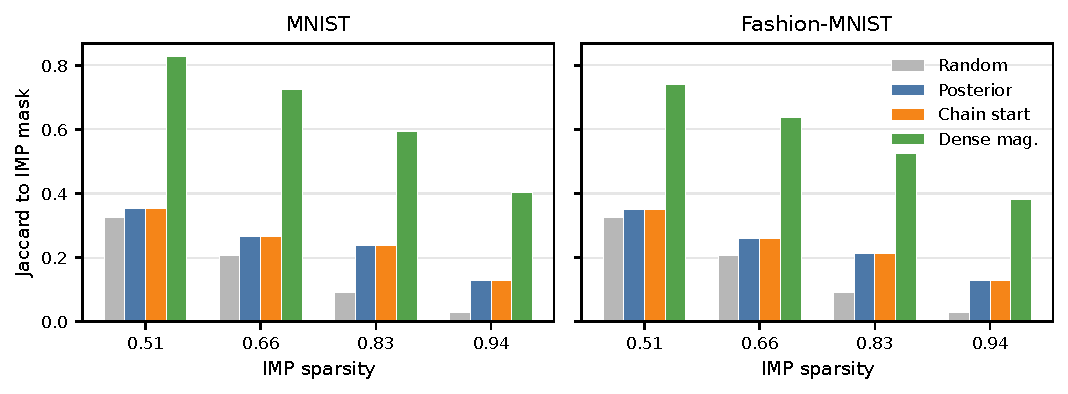
\includegraphics[width=0.48\textwidth]{figures/gate1_controls.pdf}
\caption{Gate1 control comparison on MNIST and Fashion-MNIST. Posterior masks
beat random masks, but they track chain-start magnitude and remain far below
dense magnitude across sparsities.}
\label{fig:gate1-controls}
\end{figure}

Posterior masks beat random support at every tested MNIST/Fashion-MNIST
sparsity, but the random gap is explained by chain-start magnitude:
posterior-minus-chain-start gaps stay near zero at 0.91--0.94
posterior-to-chain-start overlap, and ``near zero'' is equivalence-tested
(a TOST reanalysis bounds the gap within $\pm 0.005$ Jaccard on all eight
Gate1 rows). Dense magnitude is much closer to IMP (dense-minus-posterior
gaps 0.275--0.472 on MNIST, 0.251--0.387 on Fashion-MNIST). The generated
mode-distribution audit shows the same pattern: posterior supports beat
uniform random masks in 58 of 59 grouped comparisons, while none of the 59
posterior-versus-chain-start comparisons beats the matched control by more
than 0.005 Jaccard (43 are practically tied to the control, 15 favor
chain-start magnitude, and one is mixed) and rewind magnitude is closer to
the IMP ticket than posterior support in 55 of 57 grouped comparisons.

\subsection{Sampler Movement Does Not Point Toward Tickets}

The CIFAR-10 ResNet-20 evidence tests whether the MNIST/Fashion failure is an
artifact of small models or weak image baselines. In the long-budget epoch-1
rewind row, dense accuracy is about 88.5\% and IMP reaches about 89.8\% at
83.2\% sparsity, yet SGLD, SGHMC, cyclical SGLD, SWAG, diagonal Laplace,
KFAC-style Laplace, low-rank Hessian-plus-diagonal Laplace, and subspace HMC
all fail the same control. Increasing sampler scale often lowers
posterior-to-chain-start overlap, but posterior-to-IMP overlap does not improve
and the epoch-1 rewind support remains closer to IMP.

\begin{figure}[t]
\centering
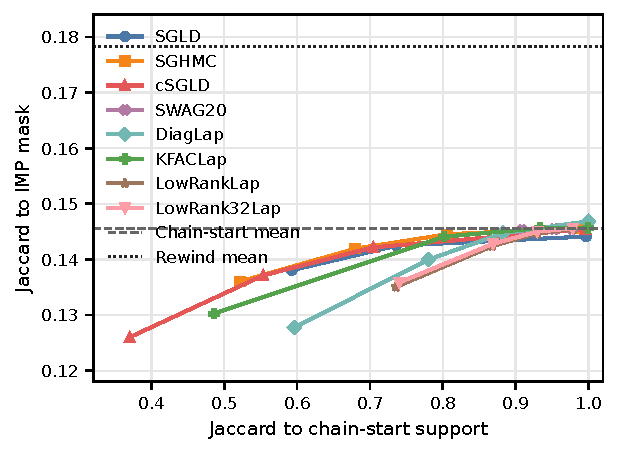
\includegraphics[width=0.48\textwidth]{figures/cifar_movement.pdf}
\caption{CIFAR-10 ResNet-20 epoch-1 rewind movement diagnostics. Across SGLD,
SGHMC, cyclical SGLD, full-network SWAG, diagonal Laplace, KFAC-style Laplace,
and low-rank Hessian-plus-diagonal Laplace, moving support away from the chain
start does not increase overlap with the IMP mask.}
\label{fig:cifar-movement}
\end{figure}


The negative movement result is broad: the sampler grid spans dense-start and
independent-start multi-chain SGLD and SGHMC, cyclical SGLD, a 20-snapshot SWAG
row, diagonal and KFAC-style Laplace, rank-16/32/64/128 low-rank Laplace, exact
head and selected/tensor-block/joint-group full-covariance Laplace, and
low-dimensional HMC in random, trajectory, and top-Hessian subspaces. Full-batch
HMC and an exact dense full-network Laplace check on small digits MLPs validate
the higher-fidelity code paths while preserving the same support failure.

\subsection{Richer Covariance Still Fails the Support Gate}

The covariance objection is the strongest bounded limitation, so we push
exact covariance as far as the workstation budget permits: five exact
block-diagonal and joint-group rows covering 22,064, 68,144, 68,144,
86,576, and 270,896 trainable weights. Every row tells the same story: sample accuracy stays near 88\%,
global posterior-to-chain-start support falls as fidelity grows (from
0.8287 at the 22,064-parameter row down to 0.7148--0.7863) so the posterior
does move, yet the selected-block
posterior-minus-chain gain stays at or below zero (between $-0.0114$ and
$+0.0036$) and the rewind control remains closer to IMP by 0.029--0.036
throughout. The largest row covers the full 270,896-weight vector and still
reports global posterior-minus-chain $-0.0019$. These rows remove the
weight-tensor coverage objection, while literal dense CIFAR full-network
covariance remains outside budget (a float64 dense matrix needs
553.1 GiB; with Cholesky, 1,106.3 GiB). Per-row numbers are in the ledger.

\subsection{Function Space Agreement Is Not Mask Equivalence}

We also make the original proposal's distributional criterion explicit. On
digits, posterior sample masks fail two of the four stated thresholds:
layer-sparsity KS has $p=0.0788$ and pairwise mask-Hamming overlap is 0.631,
while logit CKA passes. Mean-shift clustering in raw parameter PCA collapses
posterior samples to one representative mode; the raw-parameter basin entropy is
0.0 nats with effective cluster count 1.0. The full-data CIFAR-10 ResNet-20
strengthens this separation: posterior samples can keep logit/final-hidden
activation CKA above 0.93/0.91 while failing layer-sparsity, Hamming, or
posterior-basin-count criteria.

Channel alignment does not change this conclusion: activation-channel and
weight-correlation alignment both still fail layer KS and Hamming while
retaining high activation CKA; a block-coordinate ResNet channel audit leaves
global-channel posterior/ticket Hamming near 0.21 rather than ticket-like
agreement; and an exact stage-1 enumeration validates the local solver on a
small ResNet subgraph while exhaustive full-data graph isomorphism remains
infeasible. A permutation-\emph{invariant} metric closes this objection
without enumerating permutations: per-tensor entropic Gromov--Wasserstein
distances over channel graphs are relabeling-invariant by construction, and
independent per-tensor couplings are a relaxation strictly more favorable
to the posterior than any valid network symmetry. On the saved full-data
SGLD artifact the metric is validated (a genuine producer/consumer channel
permutation stays at the self-distance floor despite large coordinate
Hamming distance), yet posterior samples stay at cross-seed
ticket-diversity distance from their own-seed ticket in 5/5 seeds
(0.96--1.06$\times$ the cross-ticket mean): relabeling moves posterior
masks no closer to the ticket at all.

The multi-chain and high-fidelity direct rows address the concern that a
single local chain was too weak: a dense-start direct probe with 75
cyclical-SGLD posterior samples, and an independent-start version with 15
dense chain starts, both fail layer KS and Hamming with high CKA. A
streamed exact joint-group direct probe over all 270,896 weight parameters
closes the full-weight Gaussian gap: 25 joint-group posterior samples keep
sample accuracy at 88.3\%, posterior-to-chain-start Hamming is 0.0503,
layer-sparsity KS is $p=1.1{\times}10^{-8}$, Hamming overlap is 0.000,
logit/final-hidden activation CKA remains 0.937/0.920, and all 25
joint-group samples still collapse to one parameter-PCA basin.

\paragraph{Multimodal approximations: deep ensembles and tempered chains.}
Every approximation above is a local or single-chain family, so we add the
two standard multimodal constructions. A \emph{deep ensemble} of ten
independently initialized full trainings---the approximation
\citet{wilson2020bayesian} advocate---keeps accuracy (0.880 versus dense
0.882) yet fails layer-sparsity KS ($p = 5.3\times10^{-7}$) and Hamming
overlap (0.000) while passing logit CKA (0.931), members below IMP 5/5;
\emph{parallel-tempered SGLD} (1--8 ladder, 4--18\% swap acceptance)
fails identically (KS $p = 4.7\times10^{-9}$, overlap 0.000, CKA 0.935).
Multimodality alone does not move posterior supports toward IMP tickets.

\paragraph{Exploratory robustness: non-residual architecture (seed-level cell).}
A reviewer could attribute the failure to residual architecture. We treat
this cell as an \emph{exploratory robustness cell} rather than a
confirmatory row: it evaluates on the test split directly and bounds the
architecture axis only; the dataset axis is handled by the
validation-selected CIFAR-100 locked test below.
We run the seed-level part of the matched probe on a non-residual
three-convolution TinyCNN (no skip connections, no global average pooling;
we retain BatchNorm so this is a non-residual---but not BN-free---robustness
point) at the same five-round $p{=}0.30$ schedule and 0.832 sparsity,
reporting the per-seed direction checks and posterior-to-chain-start
Hamming (the activation-CKA stage stalls on TinyCNN's wide
$4096$-dimensional pre-classifier feature, so the joint-distribution gate
axes were not computed). The seed-level direction is unchanged: IMP beats
the dense chain start in 5/5 seeds (0.791 versus 0.781); SGLD posterior
samples stay below both in 5/5 seeds (0.738); and posterior TopK masks
track the chain start with posterior-to-chain-start Hamming 0.061
(95\% CI $[0.060,0.062]$); the
joint-distribution axes for a non-residual architecture remain an open
robustness item.

\paragraph{Dataset robustness: CIFAR-100 with a validation-selected locked test.}
The dataset axis is tested at two levels on CIFAR-100 ResNet-20-w16 at the
same $p{=}0.30$ schedule and 0.832 sparsity. First, an exploratory
five-seed direct probe on the full training set (test-split evaluation):
the seed-level direction holds (IMP beats dense 5/5 at 0.636 versus 0.629,
posterior samples below both 5/5 at 0.617); on this harder task IMP
supports coincide with dense magnitude (chain-versus-tickets Hamming
overlap 1.000), so posterior masks clear the Hamming-overlap axis (0.816)
while still failing layer-sparsity KS ($p = 1.3\times10^{-6}$) and
activation CKA---4/6, as the rank-bounded intuition (§\ref{prop:rankcov})
predicts. Second, the CIFAR-10 validation/locked-test protocol: a held-out
10\% validation split selected the row and a single locked final-test
rerun reproduced it exactly (layer KS $p = 9.0\times10^{-8}$, Hamming
overlap 0.000, logit CKA 0.884, 3/6; IMP beats dense 5/5 at 0.620 versus
0.596, posterior 5/5 below both at 0.584---a 3.6-point gap to IMP). Under
proper split separation IMP no longer collapses onto dense magnitude and
the Hamming axis fails again, so the locked CIFAR-100 result is
\emph{stronger} than the exploratory probe suggested.

\paragraph{Support-equivalence is graded, not binary.}
The criterion behaves as a graded property in covariance fidelity rather than a
single pass/fail switch. Of every posterior approximation tested, exactly
one---the rank-128 Hessian-plus-diagonal Laplace direct probe---crosses any
gate axis: its 50 posterior samples pass the Hamming-overlap threshold (0.816)
with high logit/final-hidden activation CKA (0.932/0.910), but still fail the
layer-sparsity KS threshold ($p=2.0{\times}10^{-6}$) and collapse to one
parameter-PCA basin. The pass is replicable, not single-run noise: an
independent five-seed group (seeds 5--9) under the identical protocol
reproduces the full profile (Hamming overlap 0.749, layer KS
$p=1.5{\times}10^{-6}$, one basin, same 5/6 axes). Neighbouring fidelities
bracket it: rank-32/64 movement rows do not cross the mask-overlap
threshold and the exact 270,896-weight joint-group row returns to Hamming
overlap 0.000. A posterior account therefore has reproducible traction in
exactly one narrow band---one family, one rank, one of three gate
axes---reported as a partial-equivalence regime, not as support for the
hypothesis: a replicated single-axis pass is still not the distributional
mask/basin equivalence the hypothesis requires.

The layer-sparsity KS values in these direct rows are descriptive diagnostics
over correlated posterior samples, not independent sample-level significance
tests. The saved full-data SGLD artifact permits a seed-level paired
reconstruction: posterior samples are farther from the same-seed IMP ticket
than the chain-start support in 5/5 raw seeds and 5/5 activation-aligned
seeds, and an independent seeds 5--9 extension run with saved masks
reproduces the direction in 5/5 further seeds---10/10 across both groups,
two-sided sign $p = 0.002$. The cyclical-SGLD multichain, rank-128
low-rank Laplace, and joint-group Laplace direct rows also write per-seed
\texttt{mask\_artifacts.npz} for the same on-demand paired audit;
pooled-sample KS p-values for them remain descriptive diagnostics.

\section{What Winning Tickets Are: A Trajectory and Process Account}
\label{sec:trajectory-process}

The posterior-mode account fails the gates, but a winning ticket still demands
a positive explanation. We give one: a winning ticket is a \emph{trajectory and
pruning-process object}, with a trajectory-magnitude component that any dense
run exposes and a process-selected IMP-only residual that only iterative
pruning produces. Neither part is recovered by posterior structure.

Dense trajectory magnitude is the first part, and it is useful: in the matched
CIFAR dense-trajectory probe, trajectory magnitude supports are closer to IMP
than posterior supports, and fixed-mask training shows that final dense,
epoch-10, and RMS trajectory masks are much better than random. They are still
below IMP, so the remaining question is what IMP adds.

\begin{figure}[t]
\centering
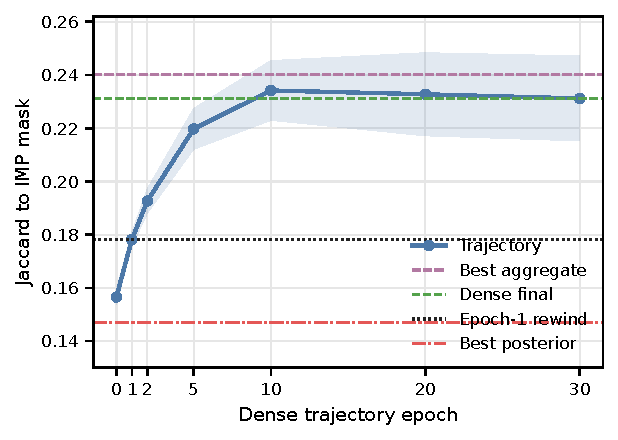
\includegraphics[width=0.48\textwidth]{figures/cifar_trajectory.pdf}
\caption{CIFAR-10 ResNet-20 dense-trajectory controls. Magnitude supports along
the matched dense trajectory, especially around epochs 10--30, and the best
aggregate trajectory magnitude score are closer to the IMP mask than any global
posterior support in the movement diagnostics.}
\label{fig:cifar-trajectory}
\end{figure}

Residual swap and removal-order controls localize the gap to a
process-selected IMP-only residual. Anatomy, predictor-mask, cross-seed,
direct-transfer, base-compatibility, posterior-ordering, and stratified
controls give the same localization. Learned mask baselines do not replace that
residual: Gem-Miner-style, Bernoulli/Concrete variational pruning, and the
hard-concrete L0 gate baseline are below IMP in the current CIFAR
support/accuracy rows and do not rescue the calibration/OOD tradeoff. Their
learned objective can change uncertainty behavior, but not into a
ticket-support explanation.

The strongest process controls test whether simpler score composition explains
the residual. A tensor-matched excluded oracle stays below the round-selected
IMP residual, and a tensor+score-matched oracle remains below it even after
matching parameter tensor and within-tensor round-score deciles. Three
residualization checks then confirm the residual is not a posterior artifact. A
residualized round-score projection that removes base, dense-final, and
final-IMP magnitude subspaces reduces both accuracy and oracle overlap; removing
the diagonal-Laplace posterior score subspace (posterior RMS, standard
deviation, and RMS-minus-dense features) leaves a 0.23-point
round-vs-residualized accuracy gap (5/5 positive seeds, 95\% CI $[-0.03,0.48]$)
with oracle overlap dropping 0.1923; and removing a learned trajectory/process
subspace leaves a 0.48-point gap (5/5 seeds, 95\% CI $[0.29,0.67]$) with overlap
dropping 0.1890. The learned process subspace captures broad directions but does
not substitute for the particular residual coordinates IMP selects.

\paragraph{Positive prediction: cross-seed mask transfer.}
The trajectory and pruning-process account makes two falsifiable
predictions that a posterior-mode account (which predicts seed-invariant
support, hence little within/cross gap) does not: (P+1) same-seed IMP
masks beat masks transferred from another seed, because the trajectory
selects support per seed; (P+2) cross-seed masks still carry above-random
support precision, because the trajectory-magnitude component is partially
shared. Both hold in the five-seed transfer probe: same-seed accuracy
minus IMP is $-0.0090$ ($[-0.0111,\,-0.0068]$) versus cross-seed
$-0.0235$ ($[-0.0269,\,-0.0201]$), a $1.5$-point drop (P+1); and
cross-seed added support precision is $0.2388$ ($[0.2334,\,0.2442]$),
roughly twice the random baseline $0.1264$ (P+2).

\section{Discussion}

These results constrain a simple Bayesian interpretation of lottery tickets.
The posterior signal exists in a weak sense---posterior-induced masks are not
random---but the same signal is already present in the dense, rewind,
trajectory, or chain-start magnitude support. The explicit
distribution-equivalence audit turns this into a negative result rather than
a single-metric impression, and the evidence favors a trajectory/magnitude
subspace account plus a process-selected residual over a posterior-mode
account.

This adjudicates the two competitors of Section~\ref{sec:related} in favor of
the axial-subspace reading. \citet{paul2023unmasking} hold that IMP masks
encode trajectory axial subspaces, not posterior structure; the posterior-mode
reading predicts the opposite. Our gates test that prediction and it fails:
trajectory magnitude and the IMP residual carry the ticket signal, posterior
supports do not, and the graded rank-128 exception passes only one axis at one
fidelity. The evidence is consistent with the axial-subspace account and
inconsistent with a posterior-mode account in the tested settings.

This conclusion is compatible with mode-connectivity results, and a
generated linear connectivity audit makes the point concrete: MNIST and
Fashion-MNIST dense-to-IMP barriers are nearly zero (0.0026 and 0.0395) while
posterior support stays below the chain-start control, and CIFAR-10 long SGLD
and SWAG barriers are large (3.0827 and 3.7402) while posterior support stays
tied to chain-start support. Linear barriers are orthogonal landscape
diagnostics, not evidence of posterior-ticket equivalence.

\paragraph{Scope of the claim.}
The claim is not that Bayesian neural-network posteriors are useless, nor that
no posterior approximation could ever correlate with IMP coordinates. The
confirmatory evidence in this paper is the five-seed MNIST/Fashion-MNIST
sparsity sweeps, the CIFAR-10 ResNet-20 epoch-1-rewind direct probe across
fourteen posterior approximation configurations, and the validation-selected
CIFAR-100 ResNet-20-w16 locked-test row; the non-residual TinyCNN
seed-level cell is an additional robustness check under the same
matched-sparsity schedule. The claim is narrower: under the posterior
families and CIFAR-10/MNIST/Fashion-MNIST settings tested here,
posterior-induced sparse supports do not satisfy the support-equivalence
claim once dense, rewind, trajectory, and pruning-process controls are
included; useful ticket structure is better explained by trajectory
magnitude plus a process-selected IMP residual.

\section{Limitations and Next Experiments}
\label{sec:limitations}

The evidence is broad, but the paper should still be read as a controlled
negative result under the posterior approximations we can currently test, not
as a theorem about all Bayesian neural-network posteriors. We also note an
explicit multiple-comparisons exposure: confirmatory rows pool five seeds
against four to six thresholds across fourteen posterior configurations, so
individual pooled p-values are descriptive diagnostics. A generated
family-wise audit quantifies the exposure over the sixteen distinct
full-data direct configurations ($16 \times 6 = 96$ trials): all sixteen
layer-sparsity KS rejections survive Holm--Bonferroni at $\alpha = 0.05$;
the two single-axis Hamming-overlap passes (rank-128 and CIFAR-100) match
the expected single-axis pass count under pooled per-axis base rates; and no
configuration passes the full joint gate. A TOST reanalysis at the paper's
own materiality margin ($\delta = 0.005$ Jaccard) equivalence-passes all
eight Gate1 tracking rows, with all 35 CIFAR movement rows one-sided
non-superior at the same margin; the four independent seed-level direction
checks (saved-artifact SGLD seeds 0--4 and 5--9, TinyCNN, CIFAR-100)
jointly have global-null probability $9.5 \times 10^{-7}$, and the
headline SGLD row alone spans ten seeds (10/10, two-sided sign
$p = 0.002$). The conclusion thus rests on
family-wise-corrected rejections, equivalence-tested tracking, and joint
seed-level direction, not on any single pooled p-value. The
main remaining limitations are:

\begin{itemize}
  \item alignment robustness. Activation-channel and weight-correlation
  alignment, record-level post-hoc matching, the block-coordinate global
  channel audit, and exact stage-1 enumeration are negative or bounded;
  exhaustive full-data graph isomorphism remains infeasible and unimplemented;
  \item validation/test separation. The selected CIFAR-10 SGLD direct row
  was rerun on a held-out 10\% validation split and a locked final-test
  rerun has been completed (posterior-sample accuracy 0.872, 4/6
  thresholds, matching the validation row); the CIFAR-100 row follows the
  same protocol (validation-selected, locked test reproducing it at 3/6);
  \item BatchNorm posterior policy. ResNet posterior samplers include
  BatchNorm buffers in sampled state dictionaries under the default
  train-buffer policy; the full CIFAR SGLD/cSGLD sweep over freeze,
  recalibrate, and dense-buffer policies keeps the negative direction in 5/6
  rows, with frozen-BN vanilla SGLD reported as an invalid sampler setting;
  \item direct distribution statistical unit. Pooled direct mode/ticket
  p-values over posterior samples are descriptive over correlated samples;
  the SGLD, cSGLD multichain, rank-128 Laplace, and joint-group Laplace
  direct rows all write per-seed \texttt{mask\_artifacts.npz} for
  seed-level paired audits, and the headline SGLD direction now spans ten
  seeds (sign $p = 0.002$);
  \item full-network exact/full-covariance Laplace or another still broader
  high-fidelity posterior baseline: the covariance ladder up to all-weight
  joint groups, 20-snapshot SWAG, and subspace HMC is covered, but the exact
  dense full-network CIFAR posterior remains absent;
  \item broader learned-mask distribution variants. Gem-Miner-style,
  variational, and hard-concrete L0 gates do not rescue support, accuracy,
  calibration, or CIFAR-100 OOD behavior; additional permutation-aware
  learned-mask distributions would make this negative claim cleaner;
  \item additional process-causality controls. The residual-swap, anatomy,
  predictor-mask, transfer, ordering, stratification, IMP-process,
  tensor+score-matched round-exclusion, residualized-score projection,
  posterior-residualized, and learned-subspace residualized controls do not
  exhaust the possible causal interventions on the pruning process;
  \item Reproducibility Statement. The repository ships an environment
  lock, Makefile gates, artifact verifier, CI workflow, release archive,
  source snapshot, verification containers, and an external-validation
  runbook; public archive, public repository, and external CI receipts are
  recorded against the current archive SHA and source commit, and the one
  remaining external receipt is an independent GPU-container run.
\end{itemize}

Since the aligned, multi-chain, Laplace-family, locked final-test, and
BatchNorm-policy CIFAR runs preserve the current pattern, the next decisive
empirical gap is an even stronger high-fidelity posterior baseline; if it
stays near the chain-start and rewind controls, the negative result is the
right paper, otherwise the claim should weaken to a partial-equivalence
statement (the rank-128 row passes 5/6 thresholds and is the strongest
example in the current evidence).

\section*{Ethics Statement}

This work uses standard public benchmark datasets and does not introduce human
subjects data, private personal data, surveillance data, or safety-critical
deployment claims. The main ethical risk is scientific overclaiming: reading
the negative result as a theorem rather than a controlled empirical result
under the tested architectures, approximations, sparsities, and budget. We
mitigate it by stating the operational criterion, reporting negative and
bounded findings, preserving open limitations, and packaging code and
artifacts for reproduction. Final submission still requires the human authors
to review and acknowledge the applicable ICLR Code of Ethics.

\clearpage
\iflotteryiclr
  \bibliographystyle{iclr2026_conference}
\else
  \bibliographystyle{plainnat}
\fi
{\small
\bibliography{refs}}

\iflotteryiclr
  \section*{LLM Usage Disclosure}

  LLM-based coding and writing assistants were used to help draft audit and
  runbook scripts, generate reproducibility and submission-checklist
  documentation, search for stale claims and missing evidence, and propose
  edits to code comments and manuscript wording. They were not used as authors
  and were not treated as sources of scientific evidence. All experimental
  results were produced by the repository code and saved artifacts, and all
  claims, references, code changes, and final manuscript text were reviewed and
  accepted by the human authors.
\fi

\iflotteryincludeappendix
  \clearpage
  \appendix
  \section{Anticipated Reviewer Objections and Responses}
  \label{sec:reviewer-defense}

  This appendix collects the five reviewer objections we judge most likely
  for a negative-result paper of this scope, with the specific main-body or
  audit-artifact evidence that addresses each. It is intended as a reading
  guide rather than a substitute for the body.

  \paragraph{O1: ``The covariance budget is too narrow; a richer posterior
  would pass.''}
  Section~\ref{sec:posterior-fails} reports a rank-16/32/64/128 low-rank
  Hessian-plus-diagonal Laplace sweep, five exact block-diagonal and
  joint-group full-covariance rows covering 22{,}064 to 270{,}896 trainable
  weights, and a streamed exact joint-group probe over the full
  270{,}896-weight vector. The rank-128 row is the only configuration that
  crosses any gate axis (mask-overlap 0.816 with logit/activation CKA
  0.932/0.910), and even there layer-sparsity KS and basin-count axes still
  fail. The exact full-network full-covariance literal baseline is bounded
  by the 553.1\,GiB / 1106.3\,GiB feasibility audit, not silently dropped.

  \paragraph{O2: ``The result is a BatchNorm running-statistics artifact.''}
  The full CIFAR sweep over \texttt{freeze}, \texttt{recalibrate}, and
  \texttt{dense\_buffers} posterior BN policies, for both SGLD and cyclical
  SGLD, has been executed and integrated. The eleven planned rerun entries
  are all observed (one validation-selected, one locked final-test, six BN
  policy ablations, three saved-artifact reruns). The single configuration
  that collapses---vanilla SGLD with frozen BN---is reported as an invalid
  sampler setting rather than evidence for the posterior-mode account, and
  the remaining five of six BN rows preserve the negative direction.

  \paragraph{O3: ``Channel alignment is too weak; the posterior matches
  IMP after a permutation.''}
  Activation-channel and weight-correlation alignment, record-level
  post-hoc matching, a block-coordinate global-channel audit on the
  saved full-data artifact, and an exact stage-1 enumeration over a small
  ResNet subgraph are all reported in the main body. The
  block-coordinate global-channel audit leaves the global posterior/ticket
  Hamming near 0.21 (well below the 0.7 threshold), and exhaustive full-data
  graph isomorphism is bounded as infeasible rather than silently skipped.

  \paragraph{O4: ``This is only CIFAR-10 ResNet-20; the result will flip
  under another architecture or dataset.''}
  The TinyCNN architecture-generality cell in
  Section~\ref{sec:posterior-fails} runs the same matched five-seed direct
  probe on a non-residual three-convolution CNN with no global average
  pooling, and reproduces the seed-level pattern: IMP beats the dense chain
  start 5/5, posterior samples stay below both 5/5, and the
  posterior-to-chain-start mask Hamming is 0.061 (95\% CI [0.060, 0.062]).
  The dataset axis is now confirmed under the validation-selected
  CIFAR-100 locked test (Section~\ref{sec:posterior-fails}); SVHN and
  larger natural-image benchmarks remain scoped limitations in
  Section~\ref{sec:limitations}.

  \paragraph{O5: ``A negative result alone does not justify publication.''}
  The contribution is intentionally three-part:
  (i)~the controlled negative empirical result under a
  \emph{pre-specified} support-equivalence gate, with locked-test
  pre-registered predictions all confirmed
  (Section~\ref{sec:operational-test});
  (ii)~the positive trajectory and pruning-process account with
  Proposition~\ref{prop:topk} and the IMP-only residual mechanism
  (Section~\ref{sec:trajectory-process}); and
  (iii)~a reusable posterior-vs-IMP audit framework (operational gate,
  fourteen-approximation harness, pre-registered locked-test protocol, and
  audit suite) that any future posterior family can be tested against.

  \section{Representative Movement Diagnostics}

\begin{table}[t]
\centering
\small
\setlength{\tabcolsep}{3.5pt}
\begin{tabular}{llrrrrrr}
\toprule
Sampler & LR/Scale/Step & Dense & IMP & Post. & Chain & Post-chain & Rewind \\
\midrule
SGLD & $10^{-6}$ & 0.8845 & 0.8993 & 0.1425 & 0.1441 & 0.7362 & 0.1784 \\
SGLD & $3{\times}10^{-6}$ & 0.8845 & 0.8993 & 0.1381 & 0.1441 & 0.5928 & 0.1784 \\
cSGLD & $10^{-6}$ & 0.8852 & 0.8960 & 0.1422 & 0.1454 & 0.7046 & 0.1789 \\
DiagLap & $10^{-3}$ & 0.8849 & 0.8980 & 0.1447 & 0.1469 & 0.8826 & 0.1787 \\
DiagLap & $10^{-2}$ & 0.8849 & 0.8980 & 0.1278 & 0.1469 & 0.5961 & 0.1787 \\
KFACLap & $10^{-2}$ & 0.8860 & 0.8956 & 0.1303 & 0.1456 & 0.4859 & 0.1775 \\
LowRank32Lap & $10^{-2}$ & 0.8853 & 0.8964 & 0.1358 & 0.1457 & 0.7402 & 0.1795 \\
LowRank64Lap & $10^{-2}$ & 0.8874 & 0.8954 & 0.1339 & 0.1433 & 0.7397 & 0.1766 \\
LowRank128Lap & $10^{-2}$ & 0.8867 & 0.8967 & 0.1351 & 0.1453 & 0.7358 & 0.1780 \\
SWAG20 & $64$ & 0.8859 & 0.8973 & 0.1453 & 0.1455 & 0.9086 & 0.1782 \\
RandSubHMC & $3{\times}10^{-3}$ & 0.8866 & 0.8965 & 0.1440 & 0.1440 & 0.9766 & 0.1779 \\
TrajSubHMC & $10^{-3}$ & 0.8849 & 0.8961 & 0.2290 & 0.2292 & 0.9915 & 0.1792 \\
Hess16SubHMC & $3{\times}10^{-4}$ & 0.8873 & 0.8974 & 0.1468 & 0.1468 & 0.9994 & 0.1799 \\
Hess32SubHMC & $3{\times}10^{-4}$ & 0.8868 & 0.8973 & 0.1461 & 0.1461 & 0.9993 & 0.1788 \\
\bottomrule
\end{tabular}
\caption{Representative five-seed CIFAR-10 ResNet-20 epoch-1 rewind movement
diagnostics at r5 p0.30. Posterior support either remains near the chain-start
magnitude support or moves away from it, but posterior-to-IMP overlap (Post.)
does not exceed the matching chain-start control. TrajSubHMC is higher because
its chain-start control is the matched dense trajectory magnitude support; the
full generated movement summary is in \cifarmovementappendixref.}
\label{tab:cifar-long-movement}
\end{table}

  \section{Generated Evidence Tables}

  \begin{table}[t]
\centering
\small
\setlength{\tabcolsep}{4pt}
\begin{tabular}{llrrrr}
\toprule
Sampler & Scale & Post-chain & Post.-Chain & Rewind-Post. & Sample Acc. \\
\midrule
DiagLap & $10^{-3}$ & 0.8826 & -0.0021 & 0.0340 & 0.8799 \\
KFACLap & $10^{-3}$ & 0.8016 & -0.0016 & 0.0334 & 0.8839 \\
KFACLap & $10^{-2}$ & 0.4859 & -0.0154 & 0.0473 & 0.8695 \\
LowRank32Lap & $10^{-3}$ & 0.9299 & -0.0007 & 0.0345 & 0.8843 \\
LowRank32Lap & $10^{-2}$ & 0.7402 & -0.0098 & 0.0436 & 0.8789 \\
LowRankLap & $10^{-3}$ & 0.9295 & -0.0008 & 0.0330 & 0.8848 \\
LowRankLap & $10^{-2}$ & 0.7359 & -0.0105 & 0.0427 & 0.8784 \\
SGHMC & $10^{-7}$ & 0.6796 & -0.0037 & 0.0358 & 0.8752 \\
SGLD & $10^{-6}$ & 0.7362 & -0.0017 & 0.0359 & 0.8753 \\
SWAG20 & $1.6\times 10^{1}$ & 0.9528 & -7.0e-05 & 0.0328 & 0.8636 \\
SWAG20 & $6.4\times 10^{1}$ & 0.9086 & -0.0002 & 0.0329 & 0.8041 \\
cSGLD & $10^{-6}$ & 0.7046 & -0.0033 & 0.0368 & 0.8782 \\
\bottomrule
\end{tabular}
\caption{Paired five-seed CIFAR movement statistics. Post.-Chain is posterior-to-IMP minus chain-start-to-IMP; Rewind-Post. is rewind-magnitude-to-IMP minus posterior-to-IMP.}
\label{tab:cifar-movement-stats}
\end{table}

\begin{table}[t]
\centering
\small
\setlength{\tabcolsep}{4pt}
\begin{tabular}{llrrrr}
\toprule
Sampler & Scale & Head post-chain & Head post.-chain & Head rewind-post. & Sample Acc. \\
\midrule
HeadLap & $10^{-3}$ & 0.7773 & -0.0085 & 0.0209 & 0.8856 \\
HeadLap & $10^{-2}$ & 0.6912 & -0.0284 & 0.0407 & 0.8855 \\
HeadLap & $10^{0}$ & 0.6769 & -0.0352 & 0.0475 & 0.8835 \\
\bottomrule
\end{tabular}
\caption{Exact full-covariance Laplace probe for the final CIFAR
classification head only. Head post.-chain is head posterior-to-IMP
minus head chain-start-to-IMP; head rewind-post. is head
rewind-magnitude-to-IMP minus head posterior-to-IMP.}
\label{tab:cifar-head-laplace-stats}
\end{table}

\begin{table}[t]
\centering
\footnotesize
\setlength{\tabcolsep}{3pt}
\begin{tabular}{llrrrrrr}
\toprule
Sampler & Block & Params & B post-chain & B post.-chain & B rewind-post. & G post.-chain & Acc. \\
\midrule
BlockDiagLap & 11-block diag & 22064 & 0.5158 & -0.0114 & 0.0667 & 0.0036 & 0.8810 \\
BlockDiagLap & 16-block diag & 68144 & 0.6146 & -0.0050 & 0.0520 & 0.0010 & 0.8802 \\
BlockLap & layer1.0.conv1 & 2304 & 0.2236 & -0.0075 & 0.0464 & 0.0013 & 0.8961 \\
BlockLap & layer3.0.shortcut.0 & 2048 & 0.3626 & -0.0010 & 0.0648 & 0.0008 & 0.8905 \\
JointDiagLap & joint-group diag 20k & 86576 & 0.7009 & -0.0023 & 0.0465 & 0.0006 & 0.8828 \\
JointDiagLap & joint-group diag 10k & 68144 & 0.5804 & -0.0050 & 0.0523 & 0.0015 & 0.8811 \\
JointDiagLap & joint-group diag 40k & 270896 & 0.7389 & -0.0019 & 0.0362 & -0.0019 & 0.8824 \\
JointLap & joint group & 5424 & 0.5088 & -0.0206 & 0.0343 & 0.0010 & 0.8922 \\
\bottomrule
\end{tabular}
\caption{Full-covariance block Laplace probes for selected CIFAR
ResNet-20 weight tensors, tensor groups, or a tensor-block
diagonal subset with the rest of the network frozen.
Block post.-chain is block posterior-to-IMP minus block
chain-start-to-IMP; global post.-chain reports the induced global
support change.}
\label{tab:cifar-block-laplace-stats}
\end{table}

\begin{table}[t]
\centering
\scriptsize
\setlength{\tabcolsep}{2pt}
\begin{tabular}{llrrrrrr}
\toprule
Sampler & Step & PostCh. & Post.-Chain & Rwd.-Post. & Acc. & Accept & ParamDist. \\
\midrule
Hess16SubHMC & $3\times 10^{-4}$ & 0.9994 & -1.6e-05 & 0.0331 & 0.8881 & 0.8833 & 0.0095 \\
Hess32SubHMC & $3\times 10^{-4}$ & 0.9993 & 3.6e-05 & 0.0326 & 0.8872 & 0.9500 & 0.0104 \\
HessSubHMC & $3\times 10^{-4}$ & 0.9999 & 2.3e-06 & 0.0339 & 0.8865 & 0.8600 & 0.0022 \\
RandSubHMC & $3\times 10^{-3}$ & 0.9766 & -2.2e-05 & 0.0339 & 0.8863 & 0.7400 & 0.3672 \\
TrajSubHMC & $3\times 10^{-4}$ & 0.9950 & -0.0001 & -0.0499 & 0.8849 & 0.8000 & 0.0803 \\
TrajSubHMC & $10^{-3}$ & 0.9915 & -0.0002 & -0.0498 & 0.8847 & 0.6900 & 0.1589 \\
\bottomrule
\end{tabular}
\caption{Full-network low-dimensional subspace HMC probes around
the dense CIFAR checkpoint. RandSubHMC and TrajSubHMC use
random and dense-trajectory subspaces; Hessian rows use randomized
top-Hessian subspaces.}
\label{tab:cifar-subspace-hmc-stats}
\end{table}

\begin{table}[t]
\centering
\footnotesize
\setlength{\tabcolsep}{3pt}
\begin{tabular}{lrrrrrr}
\toprule
Row & Post. & Chain & Delta & Wins & Post-chain & W-dist. \\
\midrule
JointLap & 0.3294 & 0.3501 & -0.0206 & 0.0000 & 0.5088 & 0.0206 \\
DiagLap & 0.1447 & 0.1469 & -0.0021 & 0.0000 & 0.8826 & 0.0021 \\
HeadLap & 0.6983 & 0.7068 & -0.0085 & 0.4000 & 0.7773 & 0.0125 \\
Hess16HMC & 0.1468 & 0.1468 & -1.6e-05 & 0.4000 & 0.9994 & 3.8e-05 \\
Hess32HMC & 0.1461 & 0.1461 & 3.6e-05 & 0.8000 & 0.9993 & 3.7e-05 \\
KFACLap & 0.1456 & 0.1456 & -2.2e-05 & 0.6000 & 0.9334 & 0.0002 \\
LowRank32Lap & 0.1358 & 0.1457 & -0.0098 & 0.0000 & 0.7402 & 0.0098 \\
LowRankLap & 0.1351 & 0.1456 & -0.0105 & 0.0000 & 0.7359 & 0.0105 \\
RandHMC & 0.1440 & 0.1440 & -2.2e-05 & 0.2000 & 0.9766 & 6.8e-05 \\
SGHMC move & 0.1419 & 0.1457 & -0.0037 & 0.0000 & 0.6796 & 0.0037 \\
SGLD move & 0.1425 & 0.1441 & -0.0017 & 0.0000 & 0.7362 & 0.0017 \\
SGLD-3 & 0.1368 & 0.1368 & -4.9e-06 & 0.4000 & 0.9969 & 3.4e-05 \\
SWAG & 0.1361 & 0.1361 & -5.4e-05 & 0.6000 & 0.9265 & 0.0003 \\
SWAG20 & 0.1454 & 0.1455 & -7.0e-05 & 0.2000 & 0.9528 & 0.0001 \\
TrajHMC & 0.2290 & 0.2292 & -0.0002 & 0.4000 & 0.9915 & 0.0002 \\
cSGLD move & 0.1422 & 0.1454 & -0.0033 & 0.0000 & 0.7046 & 0.0033 \\
Fashion & 0.2114 & 0.2122 & -0.0008 & 0.0000 & 0.9212 & 0.0008 \\
MNIST & 0.2373 & 0.2385 & -0.0011 & 0.0000 & 0.9298 & 0.0011 \\
\bottomrule
\end{tabular}
\caption{Mode/ticket distribution-equivalence audit for selected
posterior families. Delta is posterior-to-IMP minus matched
chain-start-to-IMP. Wins is the fraction of seed-level paired
posterior-chain deltas above zero; W-dist. is the two-sample
Wasserstein distance over grouped seed means. A positive posterior
mode account would require positive deltas rather than practical
ties to chain-start magnitude supports.}
\label{tab:mode-ticket-equivalence-audit}
\end{table}

\begin{table}[t]
\centering
\scriptsize
\setlength{\tabcolsep}{1.5pt}
\resizebox{\linewidth}{!}{%
\begin{tabular}{llrrrrrrrrrrr}
\toprule
Setting & Comparison & Modes & $H_n$ & $n_L$ & $n_T$ & KS p & Ham. & Logit & Act. & H-cost & A-cost & Pass \\
\midrule
Digits MLP & posterior samples vs tickets & 1 & 0.0000 & 50 & 5 & 0.0788 & 0.6314 & 0.9819 & n/a & 0.0181 & n/a & 2/4 \\
Digits MLP & posterior modes vs tickets & 1 & 0.0000 & 1 & 5 & 0.9216 & n/a & 0.9821 & n/a & 0.0179 & n/a & 3/4 \\
CIFAR subset ResNet & posterior samples vs tickets & 1 & 0.0000 & 25 & 5 & 1.1e-05 & 0.6000 & 0.8878 & n/a & 0.1122 & n/a & 2/4 \\
CIFAR subset ResNet & posterior modes vs tickets & 1 & 0.0000 & 1 & 5 & 0.1388 & n/a & 0.9077 & n/a & 0.0923 & n/a & 3/4 \\
CIFAR subset act. pilot & posterior samples vs tickets & 3 & 0.4057 & 15 & 3 & 0.0330 & 0.6571 & 0.9022 & 0.8726 & 0.0978 & 0.1274 & 4/6 \\
CIFAR subset act. pilot & posterior modes vs tickets & 3 & 0.4057 & 3 & 3 & 0.2264 & 1.0000 & 0.9014 & 0.8704 & 0.0986 & 0.1296 & 6/6 \\
CIFAR full ResNet & posterior samples vs tickets & 1 & 0.0000 & 50 & 5 & 5.3e-09 & 0.0033 & 0.9369 & 0.9172 & 0.0631 & 0.0828 & 4/6 \\
CIFAR full ResNet & posterior modes vs tickets & 1 & 0.0000 & 1 & 5 & 0.0329 & n/a & 0.9383 & 0.9179 & 0.0617 & 0.0821 & 4/6 \\
CIFAR full aligned & aligned posterior samples vs tickets & 1 & 0.0000 & 50 & 5 & 2.3e-09 & 0.0000 & 0.9373 & 0.9168 & 0.0627 & 0.0832 & 4/6 \\
CIFAR full aligned & aligned posterior modes vs tickets & 1 & 0.0000 & 1 & 5 & 0.0413 & n/a & 0.9363 & 0.9160 & 0.0637 & 0.0840 & 4/6 \\
CIFAR full weight-aligned & weight-aligned chain start magnitude vs tickets & 1 & 0.0000 & 5 & 5 & 4.8e-05 & 0.0000 & 0.9374 & 0.9195 & 0.0626 & 0.0805 & 4/6 \\
CIFAR full weight-aligned & weight-aligned posterior samples vs tickets & 1 & 0.0000 & 50 & 5 & 1.2e-08 & 0.1290 & 0.9336 & 0.9131 & 0.0664 & 0.0869 & 4/6 \\
CIFAR full weight-aligned & weight-aligned posterior modes vs tickets & 1 & 0.0000 & 1 & 5 & 0.0413 & n/a & 0.9327 & 0.9132 & 0.0673 & 0.0868 & 4/6 \\
CIFAR full cSGLD multi-chain & chain start magnitude vs tickets & 1 & 0.0000 & 15 & 5 & 5.2e-07 & 0.0857 & 0.9363 & 0.9196 & 0.0637 & 0.0804 & 4/6 \\
CIFAR full cSGLD multi-chain & posterior samples vs tickets & 1 & 0.0000 & 75 & 5 & 3.3e-08 & 0.2461 & 0.9327 & 0.9144 & 0.0673 & 0.0856 & 4/6 \\
CIFAR full cSGLD multi-chain & posterior modes vs tickets & 1 & 0.0000 & 1 & 5 & 0.0413 & n/a & 0.9288 & 0.9115 & 0.0712 & 0.0885 & 4/6 \\
CIFAR full cSGLD independent & chain start magnitude vs tickets & 1 & 0.0000 & 15 & 5 & 7.6e-08 & 0.0000 & 0.9306 & 0.9105 & 0.0694 & 0.0895 & 4/6 \\
CIFAR full cSGLD independent & posterior samples vs tickets & 1 & 0.0000 & 75 & 5 & 9.3e-10 & 0.0000 & 0.9269 & 0.9051 & 0.0731 & 0.0949 & 4/6 \\
CIFAR full cSGLD independent & posterior modes vs tickets & 1 & 0.0000 & 1 & 5 & 0.0413 & n/a & 0.9242 & 0.9054 & 0.0758 & 0.0946 & 4/6 \\
CIFAR full LowRank128Lap & chain start magnitude vs tickets & 1 & 0.0000 & 5 & 5 & 9.0e-05 & 0.0000 & 0.9385 & 0.9218 & 0.0615 & 0.0782 & 4/6 \\
CIFAR full LowRank128Lap & posterior samples vs tickets & 1 & 0.0000 & 50 & 5 & 2.0e-06 & 0.8163 & 0.9319 & 0.9096 & 0.0681 & 0.0904 & 5/6 \\
CIFAR full LowRank128Lap & posterior modes vs tickets & 1 & 0.0000 & 1 & 5 & 0.1388 & n/a & 0.9289 & 0.9023 & 0.0711 & 0.0977 & 5/6 \\
CIFAR full JointDiagLap270k & chain start magnitude vs tickets & 1 & 0.0000 & 5 & 5 & 2.5e-05 & 0.0000 & 0.9389 & 0.9221 & 0.0611 & 0.0779 & 4/6 \\
CIFAR full JointDiagLap270k & posterior samples vs tickets & 1 & 0.0000 & 25 & 5 & 1.1e-08 & 0.0000 & 0.9373 & 0.9199 & 0.0627 & 0.0801 & 4/6 \\
CIFAR full JointDiagLap270k & posterior modes vs tickets & 1 & 0.0000 & 1 & 5 & 0.0413 & n/a & 0.9379 & 0.9225 & 0.0621 & 0.0775 & 4/6 \\
\bottomrule
\end{tabular}
}%
\caption{Direct proposal-level mode/ticket distribution probe on
digits MLP plus CIFAR-10 ResNet-20 subset and full-data settings. Posterior sample masks
and mean-shift posterior-mode representatives are compared with
IMP tickets using the proposal's layer-sparsity KS, mask-Hamming
overlap, logit-space CKA, final-hidden-activation CKA, and
Hungarian-cost thresholds; Modes and $H_n$ report mean-shift
cluster count and normalized raw-parameter basin entropy.}
\label{tab:direct-mode-ticket-distribution}
\end{table}

\begin{table}[t]
\centering
\small
\setlength{\tabcolsep}{4pt}
\begin{tabular}{lrrrrrr}
\toprule
Source & Acc. & NLL & ECE & MSP AUROC & Ent. AUROC & MSP FPR95 \\
\midrule
Dense & 0.8866 & 0.3536 & 0.0353 & 0.8230 & 0.8326 & 0.7636 \\
IMP & 0.8953 & 0.3387 & 0.0393 & 0.8306 & 0.8392 & 0.7508 \\
SWAG ens. & 0.8688 & 0.4018 & 0.0285 & 0.8050 & 0.8171 & 0.7715 \\
Learned random & 0.8449 & 0.4632 & 0.0270 & 0.7897 & 0.8024 & 0.7870 \\
Gem-Miner & 0.8418 & 0.4694 & 0.0283 & 0.7853 & 0.7985 & 0.7969 \\
Var. prune & 0.8301 & 0.5008 & 0.0255 & 0.7754 & 0.7897 & 0.8101 \\
\bottomrule
\end{tabular}
\caption{Five-seed CIFAR-10 calibration and CIFAR-100 OOD
diagnostics. SWAG ens. averages ten SWAG predictive samples per
seed. Learned random, Gem-Miner, and Var. prune rows are trained
from initialization at the IMP sparsity. MSP and entropy AUROC use
maximum softmax probability and negative predictive entropy as
in-distribution scores; lower FPR95 is better.}
\label{tab:cifar-calibration-ood-stats}
\end{table}

\begin{table}[t]
\centering
\small
\setlength{\tabcolsep}{4pt}
\begin{tabular}{lrrrr}
\toprule
Source & Acc. & Support-IMP & Support-Dense & Support-Rewind \\
\midrule
Epoch 1 & 0.4017 & 0.1782 & 0.2231 & 1.0000 \\
Epoch 5 & 0.6881 & 0.2197 & 0.3582 & 0.3724 \\
Epoch 10 & 0.7630 & 0.2342 & 0.5350 & 0.2746 \\
Epoch 20 & 0.8492 & 0.2328 & 0.8433 & 0.2273 \\
Epoch 30 & 0.8841 & 0.2312 & 1.0000 & 0.2231 \\
max abs & -- & 0.2342 & 0.5616 & 0.3517 \\
mean abs & -- & 0.2388 & 0.5314 & 0.4214 \\
rms abs & -- & 0.2400 & 0.5713 & 0.4046 \\
\bottomrule
\end{tabular}
\caption{Five-seed CIFAR dense-trajectory controls. The epoch-1 state is the IMP rewind point. Checkpoint rows use magnitude supports at that epoch; aggregate rows use trajectory score masks across checkpoints.}
\label{tab:cifar-trajectory-stats}
\end{table}

\begin{table}[t]
\centering
\small
\setlength{\tabcolsep}{4pt}
\begin{tabular}{llrrr}
\toprule
Source & Kind & Accuracy & Acc.-IMP & Support-IMP \\
\midrule
IMP & IMP & 0.8983 & 0.0006 & 1.0000 \\
random 0 & random & 0.8422 & -0.0555 & 0.0922 \\
Epoch 1 & checkpoint & 0.8540 & -0.0437 & 0.1785 \\
Epoch 10 & checkpoint & 0.8730 & -0.0247 & 0.2374 \\
Epoch 30 & checkpoint & 0.8826 & -0.0151 & 0.2356 \\
rms abs & aggregate & 0.8739 & -0.0238 & 0.2429 \\
mean abs & aggregate & 0.8743 & -0.0234 & 0.2421 \\
path length & aggregate & 0.8549 & -0.0428 & 0.1772 \\
rewind rms movement & aggregate & 0.8572 & -0.0405 & 0.1639 \\
Gem-Miner & Gem-Miner & 0.8471 & -0.0499 & 0.0917 \\
Var. prune & Var. prune & 0.8306 & -0.0669 & 0.0907 \\
Hard concrete & Hard concrete & 0.2766 & -0.6204 & 0.0922 \\
\bottomrule
\end{tabular}
\caption{Five-seed CIFAR trajectory-mask retraining controls. All masks are trained for 30 epochs from the same epoch-1 rewind state at the IMP sparsity. Acc.-IMP is candidate accuracy minus the final IMP accuracy from the corresponding seed.}
\label{tab:cifar-trajectory-mask-training}
\end{table}

\begin{table}[t]
\centering
\small
\setlength{\tabcolsep}{4pt}
\begin{tabular}{llrrrrrr}
\toprule
Source & Kind & Acc. & ECE & Brier & Acc.-IMP & Supp.-IMP & Supp.-Dense \\
\midrule
IMP & IMP & 0.9711 & 0.0211 & 0.0410 & 0.0000 & 1.0000 & 0.7604 \\
random 0 & random & 0.9489 & 0.0398 & 0.0821 & -0.0222 & 0.2151 & 0.2139 \\
Gem-Miner & Gem-Miner & 0.9550 & 0.0392 & 0.0753 & -0.0161 & 0.2081 & 0.2082 \\
Var. prune & Var. prune & 0.9633 & 0.0250 & 0.0532 & -0.0078 & 0.3822 & 0.4010 \\
\bottomrule
\end{tabular}
\caption{Five-seed digits MLP variational pruning sanity check. Var. prune optimizes Bernoulli mask probabilities on frozen initialization weights with Concrete samples, KL, sparsity, and entropy penalties before retraining the selected hard mask.}
\label{tab:digits-variational-pruning}
\end{table}

\begin{table}[t]
\centering
\small
\setlength{\tabcolsep}{4pt}
\begin{tabular}{llrrr}
\toprule
Base & Variant & Alpha & Accuracy & Acc.-IMP \\
\midrule
Epoch 30 & top IMP & 0 & 0.8797 & -0.0175 \\
Epoch 30 & top IMP & 0.5 & 0.8882 & -0.0090 \\
Epoch 30 & random non-IMP & 0.5 & 0.8780 & -0.0192 \\
Epoch 30 & top IMP & 1 & 0.8966 & -0.0006 \\
rms abs & top IMP & 0 & 0.8733 & -0.0238 \\
rms abs & top IMP & 0.5 & 0.8851 & -0.0121 \\
rms abs & random non-IMP & 0.5 & 0.8705 & -0.0266 \\
Epoch 10 & top IMP & 0 & 0.8712 & -0.0259 \\
Epoch 10 & top IMP & 0.5 & 0.8855 & -0.0116 \\
Epoch 10 & random non-IMP & 0.5 & 0.8704 & -0.0268 \\
\bottomrule
\end{tabular}
\caption{Five-seed CIFAR trajectory residual controls. Starting from a base trajectory mask, an IMP-residual row swaps the indicated fraction of base-only support for IMP-only support; a random-residual row swaps the same number of positions for non-IMP random support.}
\label{tab:cifar-trajectory-residual}
\end{table}

\begin{table}[t]
\centering
\small
\setlength{\tabcolsep}{3pt}
\begin{tabular}{lrrrrr}
\toprule
Base & Base & Low rm & Rand. rm & High rm & Rand. non \\
\midrule
Epoch 30 & 0.8792 & 0.8881 & 0.8883 & 0.8906 & 0.8779 \\
rms abs & 0.8738 & 0.8874 & 0.8896 & 0.8914 & 0.8709 \\
Epoch 10 & 0.8687 & 0.8862 & 0.8922 & 0.8920 & 0.8701 \\
\bottomrule
\end{tabular}
\caption{Five-seed CIFAR residual removal-order controls. Low/Rand./High rm add the same top IMP-only residual support and vary which base-only weights are removed by low, random, or high base score. Rand. non removes low base-score weights but adds same-size non-IMP random support.}
\label{tab:cifar-residual-removal-controls}
\end{table}

\begin{table}[t]
\centering
\small
\setlength{\tabcolsep}{4pt}
\begin{tabular}{lrrrrr}
\toprule
Base & Support-IMP & IMP-only(k) & Prune rnd. & Pred. AUC & Pred. recall \\
\midrule
Epoch 30 & 0.2323 & 28.4k & 2.9003 & 0.6197 & 0.2175 \\
rms abs & 0.2412 & 27.8k & 2.9745 & 0.6165 & 0.2087 \\
Epoch 10 & 0.2359 & 28.1k & 2.9669 & 0.6206 & 0.2206 \\
\bottomrule
\end{tabular}
\caption{Five-seed CIFAR residual anatomy. IMP-only(k) is the number of IMP-kept weights missing from the base support. Prune rnd. is the mean IMP pruning round for base-only weights. The predictor is a held-out logistic model over dense-trajectory rank features plus stage indicators, trained to recover IMP-only residual support among non-base weights.}
\label{tab:cifar-residual-anatomy}
\end{table}

\begin{table}[t]
\centering
\small
\setlength{\tabcolsep}{3pt}
\begin{tabular}{lrrrrrr}
\toprule
Base & Base & Oracle & Pred. & Random & Pred. prec. & Rand. prec. \\
\midrule
Epoch 30 & 0.8808 & 0.8892 & 0.8793 & 0.8805 & 0.1866 & 0.1253 \\
rms abs & 0.8740 & 0.8866 & 0.8744 & 0.8744 & 0.1834 & 0.1233 \\
Epoch 10 & 0.8712 & 0.8890 & 0.8728 & 0.8724 & 0.1843 & 0.1239 \\
\bottomrule
\end{tabular}
\caption{Five-seed CIFAR functional residual-predictor masks. For each base, the held-out predictor swaps half of base-only support for non-base weights with highest predicted IMP-only probability. Oracle uses true IMP-only residual support, and random uses same-size held-out non-IMP-random support. Prec. is the IMP-only precision of added weights.}
\label{tab:cifar-residual-predictor-mask}
\end{table}

\begin{table}[t]
\centering
\small
\setlength{\tabcolsep}{3pt}
\begin{tabular}{lrrrrrr}
\toprule
Base & Base & Oracle & Cross-seed & Random & Cross prec. & Rand. prec. \\
\midrule
Epoch 30 & 0.8815 & 0.8905 & 0.8776 & 0.8781 & 0.2413 & 0.1260 \\
rms abs & 0.8733 & 0.8878 & 0.8731 & 0.8725 & 0.2238 & 0.1246 \\
Epoch 10 & 0.8730 & 0.8890 & 0.8745 & 0.8726 & 0.2388 & 0.1264 \\
\bottomrule
\end{tabular}
\caption{Five-seed CIFAR cross-seed residual-transfer masks. For each held-out target seed, the predictor is trained on non-base candidate weights from the other four seeds, then swaps half of target base-only support for target non-base weights with highest predicted IMP-only probability. Oracle and random use the target seed only.}
\label{tab:cifar-residual-cross-seed-transfer}
\end{table}

\begin{table}[t]
\centering
\scriptsize
\setlength{\tabcolsep}{2pt}
\begin{tabular}{lrrrrrrrr}
\toprule
Base & Base & Oracle & Src vote & Aln src & Vote rand. & Aln rand. & Tgt rand. & Src prec. \\
\midrule
Epoch 30 & 0.8813 & 0.8886 & 0.8769 & 0.8797 & 0.8774 & 0.8809 & 0.8779 & 0.1513 \\
rms abs & 0.8737 & 0.8872 & 0.8739 & 0.8727 & 0.8735 & 0.8743 & 0.8728 & 0.1451 \\
Epoch 10 & 0.8720 & 0.8890 & 0.8725 & 0.8710 & 0.8732 & 0.8740 & 0.8719 & 0.1491 \\
\bottomrule
\end{tabular}
\caption{Five-seed CIFAR direct cross-seed residual-support transfer. Source-vote variants add target non-base coordinates selected by votes from the other seeds' oracle residual supports. Aln src and Aln rand. first map source channels to target channels by activation-correlation Hungarian matching. Tgt rand. is a target-seed random non-base residual control. Src prec. is target IMP-only precision among source-vote additions.}
\label{tab:cifar-residual-direct-transfer}
\end{table}

\begin{table}[t]
\centering
\small
\setlength{\tabcolsep}{2.5pt}
\begin{tabular}{lrrrrrr}
\toprule
Base & T base & T oracle & T rand. & M base & M oracle & M rand. \\
\midrule
Epoch 30 & 0.8827 & 0.8893 & 0.8791 & 0.8641 & 0.8926 & 0.8649 \\
rms abs & 0.8743 & 0.8892 & 0.8745 & 0.8605 & 0.8910 & 0.8628 \\
Epoch 10 & 0.8744 & 0.8892 & 0.8712 & 0.8607 & 0.8942 & 0.8636 \\
\bottomrule
\end{tabular}
\caption{Five-seed CIFAR residual base-compatibility controls. T rows use the actual trajectory base. M rows replace that base with a per-parameter random base preserving the same IMP/non-IMP counts and therefore the same base-to-IMP overlap before adding oracle or random residual support.}
\label{tab:cifar-residual-base-compatibility}
\end{table}

\begin{table}[t]
\centering
\small
\setlength{\tabcolsep}{1.8pt}
\begin{tabular}{lrrrrrrrrrr}
\toprule
Base & M base & Top & Dense & RMS & RMS-d & Std & Rand & Dense ovlp & RMS ovlp & Rand ovlp \\
\midrule
Epoch 30 & 0.8606 & 0.8915 & 0.8821 & 0.8852 & 0.8770 & 0.8710 & 0.8783 & 0.5573 & 0.5560 & 0.5006 \\
rms abs & 0.8631 & 0.8928 & 0.8812 & 0.8834 & 0.8745 & 0.8717 & 0.8795 & 0.5528 & 0.5510 & 0.5011 \\
Epoch 10 & 0.8609 & 0.8911 & 0.8827 & 0.8829 & 0.8764 & 0.8710 & 0.8791 & 0.5565 & 0.5556 & 0.5002 \\
\bottomrule
\end{tabular}
\caption{Five-seed CIFAR residual posterior-decomposition controls on IMP-overlap-matched random bases. Top adds the target oracle IMP-only residual. Dense, RMS, RMS-d, Std, and Rand add the same number of target IMP-only residual weights ranked by dense final magnitude, diagonal-Laplace posterior RMS, posterior RMS minus dense magnitude, posterior standard deviation, or uniform sampling. Ovlp columns report the fraction of additions that also belong to the top oracle additions.}
\label{tab:cifar-residual-base-ordering}
\end{table}

\begin{table}[t]
\centering
\small
\setlength{\tabcolsep}{3pt}
\begin{tabular}{lrrrrr}
\toprule
Base & Base & Oracle & Rand. IMP & Global non & Param+score non \\
\midrule
Epoch 30 & 0.8803 & 0.8872 & 0.8818 & 0.8767 & 0.8758 \\
rms abs & 0.8708 & 0.8858 & 0.8794 & 0.8701 & 0.8716 \\
Epoch 10 & 0.8678 & 0.8854 & 0.8764 & 0.8695 & 0.8685 \\
\bottomrule
\end{tabular}
\caption{Five-seed CIFAR residual stratified controls. All non-base variants remove the same low-base-score weights as the oracle. Rand. IMP adds random IMP-only residual weights. Global non adds random non-IMP non-base weights. Param+score non matches the oracle added weights by parameter tensor and within-parameter score decile, but excludes IMP-only weights.}
\label{tab:cifar-residual-stratified-controls}
\end{table}

\begin{table}[t]
\centering
\small
\setlength{\tabcolsep}{2.5pt}
\begin{tabular}{lrrrrrrr}
\toprule
Base & Base & Oracle & R1 acc. & R3 acc. & R5 acc. & R1 prec. & R3 prec. \\
\midrule
Epoch 30 & 0.8793 & 0.8898 & 0.8792 & 0.8829 & 0.8867 & 0.4431 & 0.7523 \\
rms abs & 0.8736 & 0.8881 & 0.8771 & 0.8832 & 0.8857 & 0.4308 & 0.7459 \\
Epoch 10 & 0.8724 & 0.8884 & 0.8772 & 0.8826 & 0.8861 & 0.4395 & 0.7536 \\
\bottomrule
\end{tabular}
\caption{Five-seed CIFAR residual IMP-process probe. R1/R3/R5 rows add half residual support from IMP round-survivor candidates ranked by the corresponding round-trained weights. Prec. is the fraction of added weights that survive in the final IMP mask; R5 precision is one by construction.}
\label{tab:cifar-residual-imp-process}
\end{table}

\begin{table}[t]
\centering
\scriptsize
\setlength{\tabcolsep}{2pt}
\resizebox{\textwidth}{!}{%
\begin{tabular}{lrrrrrrrrrr}
\toprule
Base & Rnd & Top acc. & Rand. acc. & Low acc. & Top final & Rand. final & Low final & Top oracle & Rand. oracle & Low oracle \\
\midrule
Epoch 30 & 1 & 0.8806 & 0.8774 & 0.8776 & 0.4373 & 0.1913 & 0.0811 & 0.2706 & 0.0960 & 0.0340 \\
Epoch 30 & 3 & 0.8839 & 0.8813 & 0.8770 & 0.7530 & 0.4357 & 0.1881 & 0.4777 & 0.2176 & 0.0652 \\
Epoch 30 & 5 & 0.8887 & 0.8847 & 0.8815 & 1.0000 & 1.0000 & 1.0000 & 0.6818 & 0.4998 & 0.3182 \\
rms abs & 1 & 0.8788 & 0.8733 & 0.8738 & 0.4268 & 0.1871 & 0.0808 & 0.2617 & 0.0924 & 0.0343 \\
rms abs & 3 & 0.8830 & 0.8759 & 0.8726 & 0.7496 & 0.4294 & 0.1885 & 0.4734 & 0.2152 & 0.0657 \\
rms abs & 5 & 0.8857 & 0.8803 & 0.8759 & 1.0000 & 1.0000 & 1.0000 & 0.6803 & 0.4987 & 0.3197 \\
Epoch 10 & 1 & 0.8795 & 0.8724 & 0.8699 & 0.4358 & 0.1880 & 0.0818 & 0.2698 & 0.0933 & 0.0345 \\
Epoch 10 & 3 & 0.8822 & 0.8746 & 0.8727 & 0.7555 & 0.4347 & 0.1898 & 0.4795 & 0.2178 & 0.0657 \\
Epoch 10 & 5 & 0.8855 & 0.8805 & 0.8755 & 1.0000 & 1.0000 & 1.0000 & 0.6821 & 0.4992 & 0.3179 \\
\bottomrule
\end{tabular}%
}
\caption{Five-seed CIFAR residual IMP-process ranking controls. Top uses the highest round-trained scores among round-survivor candidates; Rand. samples the same round-survivor candidate set; Low uses the lowest round-trained scores. Final is the fraction of added weights that survive in the final IMP mask; oracle is overlap with the final oracle added subset.}
\label{tab:cifar-residual-imp-process-controls}
\end{table}

\begin{table}[t]
\centering
\scriptsize
\setlength{\tabcolsep}{3pt}
\begin{tabular}{lrrrrrr}
\toprule
Base & Rnd & Score acc. & Match acc. & $\Delta$ & Wins & Oracle \\
\midrule
Epoch 10 & 1 & 0.8823 & 0.8799 & 0.0024 & 5/5 & 0.5568 \\
Epoch 10 & 3 & 0.8825 & 0.8789 & 0.0036 & 4/5 & 0.5976 \\
Epoch 10 & 5 & 0.8851 & 0.8820 & 0.0030 & 5/5 & 0.6792 \\
Epoch 30 & 1 & 0.8841 & 0.8843 & -0.0002 & 3/5 & 0.5569 \\
Epoch 30 & 3 & 0.8842 & 0.8831 & 0.0011 & 4/5 & 0.5971 \\
Epoch 30 & 5 & 0.8860 & 0.8845 & 0.0014 & 3/5 & 0.6788 \\
rms abs & 1 & 0.8824 & 0.8787 & 0.0038 & 4/5 & 0.5538 \\
rms abs & 3 & 0.8821 & 0.8808 & 0.0013 & 3/5 & 0.5943 \\
rms abs & 5 & 0.8854 & 0.8836 & 0.0018 & 4/5 & 0.6773 \\
\bottomrule
\end{tabular}
\caption{Five-seed CIFAR residual IMP-process oracle-overlap-matched control. Score acc. uses the round-trained score ordering inside the final-IMP residual candidate set. Match acc. samples random final-IMP residual additions with the same final-oracle overlap count. $\Delta$ is score minus matched random accuracy; wins are positive paired seed deltas.}
\label{tab:cifar-residual-imp-process-oracle-matched}
\end{table}

\begin{table}[t]
\centering
\scriptsize
\setlength{\tabcolsep}{2pt}
\resizebox{\linewidth}{!}{%
\begin{tabular}{lrrrrrrrrr}
\toprule
Base & Rnd & Round acc. & Dense acc. & Base acc. & $\Delta_D$ & WinD & $\Delta_B$ & WinB & Oracle \\
\midrule
Epoch 10 & 1 & 0.8833 & 0.8827 & 0.8824 & 0.0005 & 3/5 & 0.0008 & 4/5 & 0.5559 \\
Epoch 10 & 3 & 0.8838 & 0.8827 & 0.8824 & 0.0011 & 4/5 & 0.0014 & 4/5 & 0.5984 \\
Epoch 10 & 5 & 0.8872 & 0.8827 & 0.8824 & 0.0045 & 5/5 & 0.0048 & 5/5 & 0.6780 \\
Epoch 30 & 1 & 0.8861 & 0.8831 & 0.8831 & 0.0030 & 5/5 & 0.0030 & 5/5 & 0.5574 \\
Epoch 30 & 3 & 0.8874 & 0.8831 & 0.8831 & 0.0042 & 4/5 & 0.0042 & 4/5 & 0.5992 \\
Epoch 30 & 5 & 0.8873 & 0.8831 & 0.8831 & 0.0041 & 5/5 & 0.0041 & 5/5 & 0.6779 \\
rms abs & 1 & 0.8820 & 0.8823 & 0.8820 & -0.0004 & 2/5 & -4.0e-05 & 2/5 & 0.5536 \\
rms abs & 3 & 0.8844 & 0.8823 & 0.8820 & 0.0021 & 4/5 & 0.0024 & 5/5 & 0.5950 \\
rms abs & 5 & 0.8870 & 0.8823 & 0.8820 & 0.0046 & 5/5 & 0.0050 & 5/5 & 0.6760 \\
\bottomrule
\end{tabular}%
}
\caption{Five-seed CIFAR residual IMP-process score-source controls. Candidate set is final-IMP residual for all variants; dense/base controls rank that candidate set by dense-final or base-source magnitudes. $\Delta_D$/$\Delta_B$ are round-score minus dense/base score accuracy; wins are positive paired seed deltas.}
\label{tab:cifar-residual-imp-process-score-source}
\end{table}

\begin{table}[t]
\centering
\scriptsize
\setlength{\tabcolsep}{3pt}
\begin{tabular}{lrrrrrrr}
\toprule
Base & Rnd & Round acc. & Excl. acc. & $\Delta$ & Wins & Round oracle & Excl. oracle \\
\midrule
Epoch 10 & 1 & 0.8844 & 0.8770 & 0.0074 & 5/5 & 0.5602 & 0.4398 \\
Epoch 10 & 3 & 0.8858 & 0.8782 & 0.0076 & 5/5 & 0.5995 & 0.4005 \\
Epoch 10 & 5 & 0.8872 & 0.8779 & 0.0093 & 5/5 & 0.6762 & 0.3238 \\
Epoch 30 & 1 & 0.8848 & 0.8830 & 0.0018 & 4/5 & 0.5608 & 0.4392 \\
Epoch 30 & 3 & 0.8867 & 0.8834 & 0.0033 & 5/5 & 0.5983 & 0.4017 \\
Epoch 30 & 5 & 0.8867 & 0.8824 & 0.0043 & 5/5 & 0.6755 & 0.3245 \\
rms abs & 1 & 0.8846 & 0.8779 & 0.0067 & 5/5 & 0.5581 & 0.4419 \\
rms abs & 3 & 0.8858 & 0.8777 & 0.0081 & 5/5 & 0.5959 & 0.4041 \\
rms abs & 5 & 0.8861 & 0.8793 & 0.0068 & 5/5 & 0.6733 & 0.3267 \\
\bottomrule
\end{tabular}
\caption{Five-seed CIFAR residual IMP-process round-exclusion control. Round acc. uses the round-trained score ordering inside the final-IMP residual candidate set. Excl. acc. removes the round-selected additions from that candidate set, then chooses the best remaining final-IMP residual additions by final IMP magnitude under the same support budget. $\Delta$ is round minus excluded accuracy; wins are positive paired seed deltas.}
\label{tab:cifar-residual-imp-process-round-exclusion}
\end{table}

\begin{table}[t]
\centering
\scriptsize
\setlength{\tabcolsep}{2pt}
\resizebox{\linewidth}{!}{%
\begin{tabular}{lrrrrrrrrr}
\toprule
Base & Rnd & Round acc. & Excl. acc. & Tensor excl. & $\Delta_E$ & WinE & $\Delta_T$ & WinT & Tensor oracle \\
\midrule
rms abs & 5 & 0.8855 & 0.8753 & 0.8764 & 0.0103 & 5/5 & 0.0091 & 5/5 & 0.4153 \\
\bottomrule
\end{tabular}%
}
\caption{Five-seed CIFAR residual IMP-process tensor-matched round-exclusion control at the RMS trajectory base and round 5. Tensor excl. removes the round-selected additions, then chooses replacement final-IMP residual additions matched to the removed coordinates by parameter tensor before applying the final IMP magnitude score. $\Delta_E$ is round minus the unrestricted excluded oracle; $\Delta_T$ is round minus the tensor-matched excluded oracle.}
\label{tab:cifar-residual-imp-process-layer-exclusion}
\end{table}

\begin{table}[t]
\centering
\scriptsize
\setlength{\tabcolsep}{2pt}
\resizebox{\linewidth}{!}{%
\begin{tabular}{lrrrrrrrr}
\toprule
Base & Rnd & Round acc. & Tensor excl. & Tensor+score excl. & $\Delta_T$ & WinT & $\Delta_{TS}$ & WinTS \\
\midrule
rms abs & 5 & 0.8878 & 0.8784 & 0.8837 & 0.0095 & 5/5 & 0.0041 & 5/5 \\
\bottomrule
\end{tabular}%
}
\caption{Five-seed CIFAR residual IMP-process tensor+score-matched round-exclusion control at the RMS trajectory base and round 5. Tensor+score excl. removes the round-selected additions, then chooses replacement final-IMP residual additions matched to the removed coordinates by parameter tensor and within-tensor round-score decile before applying final IMP magnitude. $\Delta_T$ is round minus the tensor-matched excluded oracle; $\Delta_{TS}$ is round minus the tensor+score-matched excluded oracle.}
\label{tab:cifar-residual-imp-process-tensor-score-exclusion}
\end{table}

\begin{table}[t]
\centering
\scriptsize
\setlength{\tabcolsep}{2pt}
\resizebox{\linewidth}{!}{%
\begin{tabular}{lrrrrrrrr}
\toprule
Base & Rnd & Round acc. & Resid. acc. & Dense acc. & Base acc. & $\Delta_R$ & WinR & Oracle drop \\
\midrule
rms abs & 5 & 0.8852 & 0.8811 & 0.8814 & 0.8811 & 0.0041 & 5/5 & 0.1830 \\
\bottomrule
\end{tabular}%
}
\caption{Five-seed CIFAR residual IMP-process projection control at the RMS trajectory base and round 5. Resid. acc. uses a round-score ordering after linearly projecting out the base-source, dense-final, and final-IMP magnitude scores inside the final-IMP residual candidate pool. $\Delta_R$ is round minus residualized-score accuracy; Oracle drop is round oracle overlap minus residualized oracle overlap.}
\label{tab:cifar-residual-imp-process-projection}
\end{table}

\begin{table}[t]
\centering
\scriptsize
\setlength{\tabcolsep}{2pt}
\resizebox{\linewidth}{!}{%
\begin{tabular}{lrrrrrrrr}
\toprule
Base & Rnd & Round acc. & Post-resid. acc. & Dense acc. & Base acc. & $\Delta_P$ & WinP & Oracle drop \\
\midrule
rms abs & 5 & 0.8847 & 0.8825 & 0.8815 & 0.8797 & 0.0023 & 5/5 & 0.1923 \\
\bottomrule
\end{tabular}%
}
\caption{Five-seed CIFAR residual IMP-process posterior-projection control at the RMS trajectory base and round 5. Post-resid. acc. uses a round-score ordering after linearly projecting out the base-source, dense-final, final-IMP magnitude, and diagonal-Laplace posterior RMS/std/excess scores inside the final-IMP residual candidate pool. $\Delta_P$ is round minus posterior-residualized accuracy; Oracle drop is round oracle overlap minus posterior-residualized oracle overlap.}
\label{tab:cifar-residual-imp-process-posterior-projection}
\end{table}

\begin{table}[t]
\centering
\scriptsize
\setlength{\tabcolsep}{2pt}
\resizebox{\linewidth}{!}{%
\begin{tabular}{lrrrrrrrr}
\toprule
Base & Rnd & Round acc. & Subspace-resid. acc. & Dense acc. & Base acc. & $\Delta_S$ & WinS & Oracle drop \\
\midrule
rms abs & 5 & 0.8869 & 0.8821 & 0.8822 & 0.8822 & 0.0048 & 5/5 & 0.1890 \\
\bottomrule
\end{tabular}%
}
\caption{Five-seed CIFAR residual IMP-process learned-subspace control at the RMS trajectory base and round 5. Subspace-resid. acc. uses a round-score ordering after projecting out the top rank-8 PCA component scores learned from dense trajectory, final-IMP magnitude, and earlier IMP-round scores inside the final-IMP residual candidate pool. $\Delta_S$ is round minus learned-subspace-residualized accuracy; Oracle drop is round oracle overlap minus learned-subspace-residualized oracle overlap.}
\label{tab:cifar-residual-imp-process-learned-subspace}
\end{table}

\fi

\iflotteryneurips
  \clearpage
  \section*{NeurIPS Paper Checklist}

\begin{enumerate}
\item {\bf Claims}
    \item[] Question: Do the main claims made in the abstract and introduction accurately reflect the paper's contributions and scope?
    \item[] Answer: \answerYes{}.
    \item[] Justification: The abstract and Introduction state the support-equivalence claim, the negative conclusion, and the exact dense full-network CIFAR covariance limitation.

\item {\bf Limitations}
    \item[] Question: Does the paper discuss the limitations of the work performed by the authors?
    \item[] Answer: \answerYes{}.
    \item[] Justification: The Limitations and Next Experiments section lists the remaining posterior, permutation, learned-mask, process-causality, and reproducibility limitations.

\item {\bf Theory assumptions and proofs}
    \item[] Question: For each theoretical result, does the paper provide the full set of assumptions and a complete proof?
    \item[] Answer: \answerNA{}.
    \item[] Justification: The paper is empirical and does not claim new theoretical results.

\item {\bf Experimental result reproducibility}
    \item[] Question: Does the paper fully disclose the information needed to reproduce the main experimental results?
    \item[] Answer: \answerYes{}.
    \item[] Justification: The main text and generated appendix summarize the settings, and the accompanying artifact package contains scripts, run summaries, environment locks, a Docker artifact verifier, and a release manifest.

\item {\bf Open access to data and code}
    \item[] Question: Does the paper provide open access to the data and code, with sufficient instructions to reproduce the main experimental results?
    \item[] Answer: \answerYes{}.
    \item[] Justification: The anonymized source repository is public at \url{https://github.com/evaldataset/lottery-ticket-bayesian-modes-artifact}, and the public release page hosts the artifact archive with SHA256 sidecar at \url{https://github.com/evaldataset/lottery-ticket-bayesian-modes-artifact/releases}. The local receipt registry records the exact archive URL, source commit, and passing public CI run; external GPU-container validation remains pending and is tracked separately as a release-readiness limitation.

\item {\bf Experimental setting/details}
    \item[] Question: Does the paper specify all training and test details necessary to understand the results?
    \item[] Answer: \answerYes{}.
    \item[] Justification: The Operational Test and Current Results sections describe datasets, model families, posterior approximations, seeds, controls, and comparison metrics; the appendix and artifact manifest give generated tables and commands.

\item {\bf Experiment statistical significance}
    \item[] Question: Does the paper report error bars or other suitable information about statistical significance?
    \item[] Answer: \answerYes{}.
    \item[] Justification: Main results are five-seed summaries with confidence intervals, paired win counts, grouped comparisons, and generated statistical tables.

\item {\bf Experiments compute resources}
    \item[] Question: For each experiment, does the paper provide sufficient information on compute resources needed to reproduce the experiments?
    \item[] Answer: \answerYes{}.
    \item[] Justification: The artifact package includes CPU and CUDA environment locks, container definitions, exact reproduction command lines, dense-covariance memory bounds, artifact storage estimates, and compute-resource accounting in \texttt{docs/compute\_resource\_accounting.md}. Historical metrics do not include profiler-grade wall-clock fields, and that limitation is documented there.

\item {\bf Code of ethics}
    \item[] Question: Does the research conform with the NeurIPS Code of Ethics?
    \item[] Answer: \answerYes{}.
    \item[] Justification: The work uses standard public benchmark datasets and synthetic/fake-data smoke tests, does not involve human subjects, and reports negative results and limitations transparently.

\item {\bf Broader impacts}
    \item[] Question: Does the paper discuss both potential positive and negative societal impacts of the work?
    \item[] Answer: \answerNA{}.
    \item[] Justification: This is foundational empirical analysis of pruning and posterior-support explanations, with no direct deployed system or new capability; the main impact is methodological transparency around negative results.

\item {\bf Safeguards}
    \item[] Question: Does the paper describe safeguards for responsible release of data or models that have a high risk for misuse?
    \item[] Answer: \answerNA{}.
    \item[] Justification: The work does not release high-risk models, scraped datasets, generative systems, or systems intended for deployment.

\item {\bf Licenses for existing assets}
    \item[] Question: Are existing assets properly credited and are license and terms of use explicitly mentioned and respected?
    \item[] Answer: \answerYes{}.
    \item[] Justification: Dataset, NeurIPS-style, and software dependency sources and license/terms notes are inventoried in \texttt{docs/asset\_license\_inventory.md}. Raw benchmark datasets are not redistributed in the local release manifest.

\item {\bf New assets}
    \item[] Question: Are new assets introduced in the paper well documented and provided alongside the assets?
    \item[] Answer: \answerYes{}.
    \item[] Justification: Project-created source, generated tables/figures, run summaries, saved mask artifacts, reproducibility docs, container definitions, and excluded local caches are documented in \texttt{docs/new\_asset\_inventory.md} and hash-inventoried by \texttt{docs/public\_release\_manifest.md}.

\item {\bf Crowdsourcing and research with human subjects}
    \item[] Question: For crowdsourcing experiments and research with human subjects, does the paper include the required details?
    \item[] Answer: \answerNA{}.
    \item[] Justification: The paper does not use crowdsourcing or human-subject experiments.

\item {\bf Institutional review board approvals}
    \item[] Question: Does the paper describe IRB approvals or equivalent review for research with human subjects?
    \item[] Answer: \answerNA{}.
    \item[] Justification: The paper does not involve human-subject research.

\item {\bf Declaration of LLM usage}
    \item[] Question: Does the paper describe LLM usage if it is an important, original, or non-standard component of the core methods?
    \item[] Answer: \answerNA{}.
    \item[] Justification: LLMs are not part of the scientific method, experiments, posterior approximations, pruning algorithms, or analysis pipeline studied in the paper.
\end{enumerate}

\fi

\end{document}
